\documentclass[11pt,a4paper]{article}

% --- Encoding and fonts ---
\usepackage[T1]{fontenc}
\usepackage[utf8]{inputenc}
\usepackage{lmodern}  % Latin Modern - clean, professional serif

% --- Math packages ---
\usepackage{amsmath}
\usepackage{amssymb}
\usepackage{amsthm}
\usepackage{mathtools}
\newcommand{\Var}{\mathrm{Var}}

% --- Layout ---
\usepackage[margin=1in]{geometry}
\usepackage{setspace}
\onehalfspacing

% --- Graphics and figures ---
\usepackage{graphicx}
\graphicspath{{../figures/}{figures/}}
\usepackage{float}
\usepackage{caption}
\usepackage{algorithm}
\usepackage{algpseudocode}
\usepackage{subcaption}
% --- Conditional compilation flags ---
% Set to \empty to include the section, \iffalse to exclude
\newif\ifincludenumerics
\newif\ifincludeempirical

% Master switches (toggle these to control output):
\includenumericstrue   % set to \includenumericsfalse to exclude Section 7
\includeempiricalfalse  % set to \includeempiricalfalse to exclude Section 8

% --- References and links ---
\usepackage[numbers,sort&compress]{natbib}
\usepackage{xcolor}
\usepackage{hyperref}
\hypersetup{
    colorlinks=true,
    linkcolor=black,
    citecolor=blue!50!black,
    urlcolor=blue!50!black
}

% --- Theorem environments ---
\theoremstyle{plain}
\newtheorem{theorem}{Theorem}[section]
\newtheorem{lemma}[theorem]{Lemma}
\newtheorem{proposition}[theorem]{Proposition}
\newtheorem{corollary}[theorem]{Corollary}

\theoremstyle{definition}
\newtheorem{definition}[theorem]{Definition}
\newtheorem{example}[theorem]{Example}
\newtheorem{remark}[theorem]{Remark}

% --- Custom commands (we'll add as needed) ---
\newcommand{\E}{\mathbb{E}}
\newcommand{\Prob}{\mathbb{P}}
\newcommand{\Q}{\mathbb{Q}}
\newcommand{\R}{\mathbb{R}}
\newcommand{\N}{\mathbb{N}}
\newcommand{\dd}{\mathrm{d}}

% --- Title block ---
\title{The Cox--Ross--Rubinstein Binomial Model:\\
       Convergence, Oscillation, and Calibration}
\author{David Dávila\thanks{I thank Dr. Hsuan-Chi Chen for his mentorship and guidance throughout this project.}\\
        \small University of New Mexico\\
        \small Department of Mathematics and Statistics}
\date{\today}

\begin{document}

\maketitle

\begin{abstract}
\noindent
This note presents a self-contained derivation of the Cox--Ross--Rubinstein
(1979) binomial option pricing model and its convergence to the
Black--Scholes formula. Great emphasis is placed on giving detailed proofs of the no-arbitrage pricing relations and deriving the risk-neutral measure through two different approaches. Additionally, we prove the convergence of the discrete-time model to its continuous-time limit using the Lindeberg--Feller central limit theorem. We then proceed to studying the non-monotone oscillation phenomenon characteristic of the standard CRR method and discuss the different smoothing alternatives of Tian (1999) and Leisen and Reimer (1996). The theoretical results are accompanied by a thorough numerical implementation in Python and C++ and an empirical calibration study using S\&P~500 index option data from OptionMetrics and Wharton Research Data Services (WRDS). Several interesting features of the convergence behavior are discussed.
\end{abstract}

\tableofcontents

\section{Introduction}
\label{sec:intro}

Option pricing theory changed fundamentally with the works of Black, Scholes, and Merton in the early 1970s. Their continuous-time framework produced the well-known and celebrated Black-Scholes formula
\[
C^{\mathrm{BS}}(S_0, K, T, r, \sigma)
= S_0 N(d_1) - K e^{-rT} N(d_2),
\]
which gives the arbitrage-free value of a European call option in terms of the spot price $S_0$, strike $K$, time to expiration $T$, risk-free rate $r$, and the volatility $\sigma$. 

The original derivation, however, relies on continuous-time stochastic calculus, It\^o's formula, and partial differential equations---tools not available to economists and finance practitioners at the time. While mathematically elegant, this advanced framework can obscure the underlying economic structure of the pricing argument. 

A few years later, Cox, Ross, and Rubinstein~(1979) introduced a discrete-time alternative based on a multiplicative binomial tree. In their model, the stock price moves up or down by fixed factors at each trading period (random walk), and option values are obtained through replication and backward induction. As the number of periods $N$ tends to infinity, the binomial price converges to the Black--Scholes price.

Today, the CRR binomial model remains one of the standard introductions to arbitrage-free pricing because it isolates the main ideas of the theory in an elementary one-period setting: replication, no-arbitrage pricing, risk-neutral probabilities, and martingale methods all appear in a finite-state form before moving to continuous-time pricing.

This note develops the CRR model from first principles, followed by a study of its convergence to Black--Scholes, both mathematically and empirically. We give particular attention to the oscillatory convergence behavior of the standard CRR tree and to the smoothing schemes introduced by Tian~(1999) and Leisen--Reimer~(1996) and its effects on oscillation behavior.

\subsection{Scope and Contribution}

This mathematical note presents a self-contained treatment of the Cox-Ross-Rubinstein binomial model and its convergence to the Black-Scholes formula.

The exposition focuses on three main points. First, we derive the discrete-time pricing framework directly from replication and no-arbitrage conditions, showing how the risk-neutral measure and martingale pricing emerge in a finite-state setting. Second, we give a mathematically detailed proof of convergence to Black--Scholes using the Lindeberg--Feller central limit theorem for triangular arrays (Theorem~\ref{thm:CRR-to-BS}). Third, we study the oscillatory convergence behavior of the standard CRR scheme and discuss the smoothing approaches of Tian~(1999) and Leisen--Reimer ~(1996).

I aim for the level of rigor appropriate to a graduate-level expository note: every theorem is stated precisely, every proof is given in detail or
referenced explicitly, and every numerical claim is grounded either in
demonstrated theory or in computations available in the accompanying coding
implementation. The exposition draws particularly on the original CRR
paper, on Shreve's~(2004) treatment in \emph{Stochastic Calculus for
Finance~II}, and on the recent classroom notes of
Chen~(2016, 2018) and Chen and Chen~(2025) on elementary derivations
of the constants appearing in the Black--Scholes formula.

The note's primary content lies in three contributions. The first is a
detailed proof of CRR's convergence theorem
(Theorem~\ref{thm:CRR-to-BS}) via the Lindeberg--Feller central limit
theorem for triangular arrays, with the explicit verification of every
step that is shown in the original paper. The second is a detailed
exposition of the oscillation phenomenon (Section~\ref{sec:oscillation}): the well-documented but often under-discussed observation that CRR convergence to Black--Scholes is not monotone in $N$, exhibiting period-2 oscillations with an $O(1/N)$
envelope. We also discuss the mechanism (the misalignment between the
strike $K$ and the terminal binomial nodes), state carefully the 
asymptotic expansion of Diener and Diener~(2004), and review the
smoothing alternatives of Tian~(1999) and Leisen and
Reimer~(1996). \ifincludenumerics
\ifincludeempirical
The third is a numerical implementation and an
empirical calibration study using historical S\&P~500 index option
data from OptionMetrics, presented in
Sections~\ref{sec:numerics} and~\ref{sec:empirical}.
\fi
\fi

\textbf{Note 1}: I make no claim of original mathematical results or findings. In fact, the CRR model and
its convergence are foundational and well-known; the oscillation
phenomenon and its asymptotic expansion are widely used in the
literature; and the Tian and Leisen--Reimer schemes are standard tools used by practitioners in the space. 
The contribution of this note is thus expository: a unified, self-contained, and mathematically careful presentation of main derivatives topics in a single document, with proofs filled in where standard references skip them, and with numerical and empirical evidence provided alongside the theory. This last part is where the main derivations come to life.

\textbf{Note 2}: The treatment of Tian~(1999) in Section~\ref{subsec:tian} is a
revision of an earlier draft. The accompanying coding implementation now
follows the construction of Tian~(1999) eqs.~(6) and~(13) directly,
verified against the paper's Tables~I and~II to four-to-six decimal
places, with the smoothing Richardson extrapolation of
eq.~(17) provided as a separate resource. Later, we will observe the implementation of both methods and their different behavior when it comes to pricing error estimation.

\textbf{Note 3} (methodology): The mathematical derivations in this note are the author's own; complete handwritten worksheets for the principal derivations (one-period replication, the closed-form CRR formula, CRR parameter asymptotics, the mean and variance of $Z_N$, the Lindeberg--Feller verification, binomial tail convergence, stock-numeraire convergence, and the oscillation mechanism) are available in the project repository. AI-assisted tools were used for prose polish, LaTeX typesetting, and figure-script structure.

The handwritten derivations underlying Sections~\ref{subsec:contingent}, 
\ref{subsec:closed-form}, \ref{subsec:crr-param}, \ref{subsec:mean-var}, 
\ref{subsec:triangular-clt}, \ref{subsec:tail-convergence}, 
\ref{subsec:p-prime}, and~\ref{subsec:oscillation-mechanism} are 
available in the project repository at 
\href{https://github.com/daviddavilad/option-pricing/blob/main/notes/CRR_Handwritten_Derivations.pdf}{notes/CRR\_Handwritten\_Derivations.pdf}.

\subsection{Connection to Earlier Work in This Series}

The constants $\sqrt{2\pi}$ and the standard normal CDF (Cumulative Distribution Function) that appear in
the Black--Scholes formula have, in fact, several routes to elementary
derivation. Newton's semicircle produces a geometric construction of the
Gaussian integral, presented in Chen~(2016); the bounds
$(1 - x/n)^n \leq e^{-x} \leq (1 + x/n)^{-n}$, applied to the
probability integral, yield Wallis's product and the
$\sqrt{\pi}/2$ value, presented in Chen~(2018); and Taylor's formula
with integral remainder produces the beta-gamma function identity, which
presented in Chen and Chen~(2025). Each derivation uses only
single-variable calculus, thus avoiding the multivariable polar-coordinate
argument typical of textbook methods. The convergence proof of
this note connects to that program in
Section~\ref{subsec:probability-integral}: the discrete-to-continuous
limit established by the Lindeberg--Feller theorem is, by its nature,
the statement that binomial tail probabilities converge to standard
normal tail probabilities, and the constant $\sqrt{2\pi}$ that
normalizes the Gaussian density is the same constant that those
elementary derivations evaluate. The present note may therefore be read as
a discrete-time alternative to the analytic derivations in that mentioned
sequence. The same constants appear, but they emerge from a probabilistic
limit theorem rather than from analytic identities.

\subsection{Organization}

Section~\ref{sec:one-period} defines and develops the one-period two-state model,
deriving the unique no-arbitrage price of a contingent claim and the
risk-neutral probability. Section~\ref{sec:n-period} extends the same 
analysis to $N$ periods, deriving the closed-form CRR pricing formula
for European calls through backward induction.
Section~\ref{sec:american} deals with American options and the
optimal-stopping problem, including the early-exercise boundary and
the adjustments required to handle dividends.
Section~\ref{sec:convergence} contains the main
mathematical result: a complete proof that the CRR price converges to
the Black--Scholes formula as $N \to \infty$, via the
Lindeberg--Feller central limit theorem.
Section~\ref{sec:oscillation} characterizes the oscillation
phenomenon and reviews the smoothing schemes of Tian and
Leisen--Reimer. \ifincludenumerics
Section~\ref{sec:numerics} presents algorithmic
details and convergence experiments.
\fi
\ifincludeempirical
Section~\ref{sec:empirical} reports the empirical calibration study
on SPX index options, using WRDS data.
\fi Section~\ref{sec:conclusion} concludes and
discusses planned extensions of this work.

\subsection{Notation and Conventions}

It is important to note that we adopt the following conventions throughout. Time is denoted $t$ in continuous-time contexts and $n$ in discrete-time contexts; horizons
are $T$ and $N$ respectively, with $\Delta t = T/N$. The risk-free
gross return is $R = e^{r \Delta t}$ over one period in the
discrete-time setting and $e^{rT}$ over the full horizon $T$ in the
continuous-time setting. The physical (real-world) probability measure
is $\Prob$; the risk-neutral measure is $\Q$, and expectations under
each are denoted $\E$ and $\E^{\Q}$ respectively. The standard normal
CDF is $N(\cdot)$, in keeping with finance convention; we use $N$ for
the number of binomial periods, but it is clarified to avoid confusion depending on the context.
The complementary binomial distribution function is denoted
$\Phi(a; N, p)$, defined in equation~\eqref{eq:def-Phi}, and must not
be confused with the standard normal CDF $N(\cdot)$. Throughout, log
means natural log.

\section{The One-Period Binomial Model}
\label{sec:one-period}

Let us begin the simplest non-trivial setting. Suppose we have a market with a single risky asset, a risk-free bond (yielding the risk-free rate), and a single period of trading. Despite its simplicity, this model contains every essential idea of arbitrage-free option pricing. The risk-neutral measure, the replicating portfolio, and the independence of option value from physical probabilities all begin here. The multi-period and continuous-time models that follow this setting are, in a precise sense, iterated and limiting versions of the same idea.

\subsection{The Market}
\label{subsec:market}

Fix a probability space $(\Omega, \mathcal{F}, \Prob)$ with two states,
$\Omega = \{\omega_u, \omega_d\}$, equipped with the physical (or
\emph{real-world}) probability measure $\Prob$ assigning
$\Prob(\omega_u) = q$ and $\Prob(\omega_d) = 1-q$ for some $q \in (0,1)$.
The market consists of two assets traded at times $t = 0$ and $t = 1$:

\begin{enumerate}
    \item A \emph{risk-free bond} with price $B_0 = 1$ at time $0$ and
    $B_1 = R$ at time $1$, where $R = 1 + r_f > 0$ and $r_f$ denotes the
    one-period risk-free rate. The bond's terminal value is deterministic.

    \item A \emph{risky asset} (``stock'') with price $S_0 = S > 0$ at
    time $0$. Its time-$1$ price $S_1$ takes two values:
    \[
    S_1(\omega) =
    \begin{cases}
        uS & \text{if } \omega = \omega_u, \\
        dS & \text{if } \omega = \omega_d,
    \end{cases}
    \]
    where $0 < d < u$ are the gross returns in the two states.
\end{enumerate}

We must impose throughout the no-arbitrage condition
\begin{equation}
    \label{eq:no-arb-1period}
    d < R < u.
\end{equation}
Its necessity is established in the following lemma.

\begin{lemma}[No-arbitrage condition]
\label{lem:no-arb}
The one-period market admits no arbitrage if and only if $d < R < u$.
\end{lemma}

\begin{proof}
Suppose first that $R \leq d$. Then borrowing one dollar at the risk-free
rate and investing in the stock yields a portfolio with time-$1$ value
$S_1 - R \geq dS - R \geq 0$ in every state, with strict inequality in
state $\omega_u$ since $u > d \geq R$. This is an arbitrage. Symmetrically,
if $R \geq u$, shorting the stock and investing the proceeds in the bond
produces an arbitrage. Conversely, suppose $d < R < u$. Any portfolio
$(\Delta, B)$ consisting of $\Delta$ shares and $B$ dollars in the bond
has time-$0$ value $\Delta S + B$ and time-$1$ values
$\Delta u S + RB$ and $\Delta d S + RB$. If both terminal values are
non-negative and at least one is positive, then $\Delta S + B > 0$,
as may be verified by considering the cases $\Delta \geq 0$ and $\Delta < 0$
separately and using $d < R < u$. Hence no arbitrage exists.
\end{proof}

\subsection{Contingent Claims and Replication}
\label{subsec:contingent}

A \emph{contingent claim} maturing at time $1$ is any random variable
$X : \Omega \to \R$, specified by its payoffs $X_u := X(\omega_u)$ and
$X_d := X(\omega_d)$. The European call option with strike $K$ corresponds
to $X = (S_1 - K)^+$, so $X_u = (uS - K)^+$ and $X_d = (dS - K)^+$.
The European put corresponds to $X = (K - S_1)^+$.

\begin{definition}[Replicating portfolio]
\label{def:replicating}
A \emph{replicating portfolio} for a claim $X$ is a pair $(\Delta, B) \in
\R^2$ satisfying
\begin{equation}
    \label{eq:replication}
    \Delta \cdot uS + RB = X_u, \qquad \Delta \cdot dS + RB = X_d.
\end{equation}
\end{definition}

The system~\eqref{eq:replication} is linear in $(\Delta, B)$ with
determinant $(u-d)RS \neq 0$, so a unique replicating portfolio exists for
every claim. Solving:
\begin{equation}
    \label{eq:delta-B}
    \Delta = \frac{X_u - X_d}{(u-d)S}, \qquad
    B = \frac{1}{R} \cdot \frac{u X_d - d X_u}{u - d}.
\end{equation}
The quantity $\Delta$ is the \emph{hedge ratio}: the number of shares
required to replicate one unit of the claim.

\begin{theorem}[One-period pricing formula]
\label{thm:one-period-pricing}
Under the no-arbitrage condition~\eqref{eq:no-arb-1period}, the unique
arbitrage-free time-$0$ price of any contingent claim $X$ is
\begin{equation}
    \label{eq:one-period-price}
    V_0 = \Delta S + B = \frac{1}{R}\bigl[ p\, X_u + (1-p)\, X_d \bigr],
\end{equation}
where
\begin{equation}
    \label{eq:risk-neutral-prob}
    p := \frac{R - d}{u - d}.
\end{equation}
\end{theorem}

\begin{proof}
Suppose the claim trades at price $V_0' \neq \Delta S + B$. If
$V_0' > \Delta S + B$, sell the claim, buy the replicating portfolio, and
invest the difference $V_0' - (\Delta S + B) > 0$ in the bond; at time $1$
the portfolio's payoff exactly cancels the claim's, leaving a riskless
profit of $R(V_0' - (\Delta S + B)) > 0$. If $V_0' < \Delta S + B$, reverse
the position. Either case contradicts no-arbitrage, so $V_0 = \Delta S + B$.
Substituting~\eqref{eq:delta-B} and simplifying:
\[
\Delta S + B
= \frac{X_u - X_d}{u - d} + \frac{1}{R} \cdot \frac{u X_d - d X_u}{u - d}
= \frac{1}{R} \left[ \frac{R(X_u - X_d) + u X_d - d X_u}{u - d} \right].
\]
The numerator equals $(R - d) X_u + (u - R) X_d$, giving
\eqref{eq:one-period-price} with $p$ as in~\eqref{eq:risk-neutral-prob}.
\end{proof}

By condition~\eqref{eq:no-arb-1period}, $p \in (0, 1)$. We may therefore
interpret $p$ as a probability and define a new measure $\Q$ on $\Omega$
by $\Q(\omega_u) = p$, $\Q(\omega_d) = 1-p$. Under $\Q$, the expected
gross return on the stock equals $R$:
\[
\E^{\Q}[S_1] = p \cdot uS + (1-p) \cdot dS
= S \cdot \frac{(R-d)u + (u-R)d}{u-d} = RS.
\]
We call $\Q$ the \emph{risk-neutral measure} (or
\emph{equivalent martingale measure}, since the discounted price
$S_t / R^t$ is a $\Q$-martingale). The pricing
formula~\eqref{eq:one-period-price} thus reads
\begin{equation}
    \label{eq:risk-neutral-pricing}
    V_0 = \frac{1}{R} \E^{\Q}[X],
\end{equation}
the discounted risk-neutral expectation of the payoff. Three features of
this result deserve emphasis.

\begin{remark}
The physical probability $q$ does not appear in
\eqref{eq:one-period-price}. Investors who disagree about the likelihood of
upward and downward moves nonetheless agree on the option's price. Pricing
is determined entirely by the absence of arbitrage and the no-arbitrage
parameters $u$, $d$, $R$.
\end{remark}

\begin{remark}
The derivation makes no assumption about investor preferences beyond
non-satiation (preferring more wealth to less, in order to exploit
arbitrage). In particular, no utility function or risk-aversion parameter
enters the pricing formula.
\end{remark}

\begin{remark}
Although $\Q$ is constructed from the no-arbitrage parameters rather than
from any economic primitive, it admits a natural interpretation: $\Q$ is
the unique probability measure equivalent to $\Prob$ under which the
discounted stock price is a martingale. This martingale property
generalizes to the multi-period and continuous-time settings and underlies
the modern formulation of arbitrage pricing due to Harrison and
Kreps~(1979) and Harrison and Pliska~(1981).
\end{remark}

\subsection{An Alternative Derivation via Binary Claims}
\label{subsec:orosi}

The replicating-portfolio argument above is standard but, as
Orosi~(2015) observes, it bundles two distinct ideas: the existence of a
replicating portfolio and the resulting risk-neutral probability. The
following alternative derivation isolates the second idea by pricing a
single elementary claim, the \emph{binary call}, and recovering $p$
directly. We include it both for its pedagogical clarity and because the
binary-claim viewpoint generalizes cleanly to the multi-period setting.

Let $\mathbf{1}_u$ denote the binary claim paying one unit in state
$\omega_u$ and zero in state $\omega_d$. By
Theorem~\ref{thm:one-period-pricing} with $X_u = 1$, $X_d = 0$, its price is
\begin{equation}
    \label{eq:binary-price}
    V_0(\mathbf{1}_u) = \frac{1}{R} \cdot \frac{R - d}{u - d} = \frac{p}{R}.
\end{equation}
The price $p/R$ has a transparent interpretation: it is the discounted
probability of the up state under $\Q$. By symmetry,
$V_0(\mathbf{1}_d) = (1-p)/R$. Any claim $X$ may be decomposed as
$X = X_u \mathbf{1}_u + X_d \mathbf{1}_d$, and linearity of pricing yields
\eqref{eq:one-period-price} immediately. The binary claims
$\mathbf{1}_u, \mathbf{1}_d$ are sometimes called \emph{Arrow--Debreu
securities} for the two states; their prices, $p/R$ and $(1-p)/R$, are the
state prices.

\subsection{An Example}
\label{subsec:example-1period}

Following Cox, Ross, and Rubinstein~(1979), consider a stock with
$S = 50$, $u = 2$, $d = 1/2$, and a one-period risk-free rate giving
$R = 5/4$. A European call with strike $K = 50$ has payoffs $C_u = 50$
and $C_d = 0$. Then
\[
p = \frac{R - d}{u - d} = \frac{5/4 - 1/2}{2 - 1/2} = \frac{1}{2},
\]
and the call's price is
\[
C_0 = \frac{1}{R}\bigl[p \cdot 50 + (1-p) \cdot 0\bigr]
    = \frac{4}{5} \cdot 25 = 20.
\]
The replicating portfolio holds $\Delta = (50 - 0) / ((2 - 1/2) \cdot 50)
= 2/3$ shares and borrows $B = -(1/R)(d C_u - u C_d)/(u - d) =
-(4/5)(25/(3/2)) = -40/3$. One verifies directly that this portfolio
delivers $50$ in state $\omega_u$ and $0$ in state $\omega_d$, matching
the call's payoff in each state.

\section{The N-Period Binomial Model}
\label{sec:n-period}

We now extend the one-period model to a finite-horizon discrete-time
setting with $N$ trading periods. The underlying logic is unchanged: at
each node of the resulting tree, the one-period analysis of
Section~\ref{sec:one-period} applies locally. What is new is the
\emph{recursive} structure of pricing, the closed-form expression for
European claims, and the explicit appearance of the binomial distribution
in the pricing formula.

\subsection{The Multiplicative Binomial Tree}
\label{subsec:tree}

Fix a horizon of $N$ periods, each of length $\Delta t > 0$. The stock
price evolves on a recombining binomial tree: at each node, the price
either multiplies by $u$ (with $\Prob$-probability $q$) or by $d$ (with
$\Prob$-probability $1-q$), independently across periods. After $j$
upward moves and $N - j$ downward moves, the time-$N$ price equals
$u^j d^{N-j} S_0$. Because the tree recombines---i.e., $ud = du$---the
order of the moves is immaterial, and the time-$N$ price depends only on
the total number of upward moves $J_N \in \{0, 1, \dots, N\}$.

We retain the one-period risk-free gross return $R = 1 + r_f > 0$,
constant across periods, and the no-arbitrage condition
$d < R < u$. Let $\Q$ denote the measure under which $\Q(\text{up}) = p$
and $\Q(\text{down}) = 1-p$ at each node, with
\[
p = \frac{R - d}{u - d} \in (0,1)
\]
as in~\eqref{eq:risk-neutral-prob}. Under $\Q$, the upward-move counts
$J_N$ follow a binomial distribution with parameters $N$ and $p$.

\subsection{Recursive Pricing}
\label{subsec:recursive}

Let $V_n(j)$ denote the time-$n$ price of a European claim $X$ at the node
reached by $j$ upward moves out of $n$, for $n = 0, 1, \dots, N$ and
$j = 0, 1, \dots, n$. At maturity,
\begin{equation}
    \label{eq:terminal}
    V_N(j) = X(u^j d^{N-j} S_0), \qquad j = 0, 1, \dots, N.
\end{equation}
At any earlier node, the one-period pricing
formula~\eqref{eq:one-period-price} applied locally yields
\begin{equation}
    \label{eq:backward}
    V_n(j) = \frac{1}{R}\bigl[ p\, V_{n+1}(j+1) + (1-p)\, V_{n+1}(j) \bigr].
\end{equation}
Equation~\eqref{eq:backward} is the \emph{backward induction} or
\emph{dynamic programming} relation for European claims. Together
with~\eqref{eq:terminal}, it determines $V_n(j)$ at every node, and in
particular determines the time-$0$ price $V_0 = V_0(0)$.

\begin{theorem}[N-period European pricing formula]
\label{thm:n-period-pricing}
The arbitrage-free time-$0$ price of a European claim $X$ with maturity
$N$ is
\begin{equation}
    \label{eq:n-period-price}
    V_0 = \frac{1}{R^N} \sum_{j=0}^{N} \binom{N}{j} p^j (1-p)^{N-j}\,
          X(u^j d^{N-j} S_0).
\end{equation}
\end{theorem}

\begin{proof}
We prove~\eqref{eq:n-period-price} by induction on $N$. The case $N = 1$
is Theorem~\ref{thm:one-period-pricing}. Suppose~\eqref{eq:n-period-price}
holds for some horizon $N \geq 1$, and consider a claim with horizon
$N+1$. Applying~\eqref{eq:backward} at time zero and the inductive
hypothesis to the two subtrees rooted at $(1,1)$ and $(1,0)$:
\[
V_0 = \frac{1}{R}\bigl[ p\, V_1(1) + (1-p)\, V_1(0) \bigr],
\]
where, by hypothesis,
\begin{align*}
V_1(1) &= \frac{1}{R^N} \sum_{k=0}^{N} \binom{N}{k} p^k (1-p)^{N-k}\,
         X(u^{k+1} d^{N-k} S_0), \\
V_1(0) &= \frac{1}{R^N} \sum_{k=0}^{N} \binom{N}{k} p^k (1-p)^{N-k}\,
         X(u^{k} d^{N-k+1} S_0).
\end{align*}
Substituting and reindexing the first sum with $j = k+1$:
\[
V_0 = \frac{1}{R^{N+1}} \sum_{j=0}^{N+1} c_j\, X(u^j d^{N+1-j} S_0),
\]
where, for $1 \leq j \leq N$,
\[
c_j = p \cdot \binom{N}{j-1} p^{j-1}(1-p)^{N-j+1}
    + (1-p) \cdot \binom{N}{j} p^j (1-p)^{N-j}
    = \binom{N+1}{j} p^j (1-p)^{N+1-j},
\]
using Pascal's identity $\binom{N+1}{j} = \binom{N}{j-1} + \binom{N}{j}$.
The boundary cases $j = 0$ and $j = N+1$ are verified directly. This
yields~\eqref{eq:n-period-price} for horizon $N+1$.
\end{proof}

Equivalently, in the notation of risk-neutral expectation,
\begin{equation}
    \label{eq:risk-neutral-N}
    V_0 = \frac{1}{R^N} \E^{\Q}[X(S_N)].
\end{equation}

\subsection{The Closed-Form Call Pricing Formula}
\label{subsec:closed-form}

For a European call with strike $K$, the payoff is $X(s) = (s - K)^+$.
Substituting into~\eqref{eq:n-period-price}:
\begin{equation}
    \label{eq:call-sum}
    C_0 = \frac{1}{R^N} \sum_{j=0}^{N} \binom{N}{j} p^j (1-p)^{N-j}\,
          (u^j d^{N-j} S_0 - K)^+.
\end{equation}
The summand is positive precisely when $u^j d^{N-j} S_0 > K$, equivalently
\[
j \log(u/d) > \log(K / (d^N S_0)),
\]
or $j > \log(K / (d^N S_0))/\log(u/d)$, since $\log(u/d) > 0$. Define
\begin{equation}
    \label{eq:def-a}
    a := \min\left\{ j \in \{0, 1, \dots, N+1\} :
              u^j d^{N-j} S_0 > K \right\},
\end{equation}
the smallest non-negative integer $j$ for which the option finishes in
the money. (If no such $j \leq N$ exists, the option expires worthless and
$C_0 = 0$; we set $a = N+1$ in this case.) Then~\eqref{eq:call-sum}
becomes
\begin{equation}
    \label{eq:call-truncated}
    C_0 = \frac{1}{R^N} \sum_{j=a}^{N} \binom{N}{j} p^j (1-p)^{N-j}
          \bigl( u^j d^{N-j} S_0 - K \bigr).
\end{equation}

We split the sum into stock and strike components. Define the
complementary binomial distribution function
\begin{equation}
    \label{eq:def-Phi}
    \Phi(a; N, \pi) := \sum_{j=a}^{N} \binom{N}{j} \pi^j (1-\pi)^{N-j},
\end{equation}
the probability that a $\mathrm{Binomial}(N, \pi)$ random variable takes
a value of at least $a$. The strike-component sum
in~\eqref{eq:call-truncated} is precisely $\Phi(a; N, p) \cdot K / R^N$.
For the stock component, define
\begin{equation}
    \label{eq:def-p-prime}
    p' := \frac{u}{R} \cdot p.
\end{equation}
We claim $p' \in (0,1)$. Positivity is immediate. For $p' < 1$, observe
that $1 - p' = (d/R)(1-p)$, since
\[
\frac{u}{R} p + \frac{d}{R}(1-p)
= \frac{up + d(1-p)}{R}
= \frac{u(R-d) + d(u-R)}{R(u-d)}
= \frac{R(u-d)}{R(u-d)} = 1.
\]
Thus $1 - p' = (d/R)(1-p) > 0$, so $p' < 1$. Now the stock-component sum
satisfies
\begin{align*}
\frac{1}{R^N} \sum_{j=a}^{N} \binom{N}{j} p^j (1-p)^{N-j}\, u^j d^{N-j} S_0
&= S_0 \sum_{j=a}^{N} \binom{N}{j} \left(\frac{up}{R}\right)^j
        \left(\frac{d(1-p)}{R}\right)^{N-j} \\
&= S_0 \sum_{j=a}^{N} \binom{N}{j} (p')^j (1-p')^{N-j}
= S_0 \, \Phi(a; N, p').
\end{align*}
Combining, we obtain the binomial call pricing formula.

\begin{theorem}[Cox--Ross--Rubinstein, 1979]
\label{thm:CRR-formula}
The arbitrage-free time-$0$ price of a European call option with strike
$K$ and maturity $N$ in the binomial model is
\begin{equation}
    \label{eq:CRR-formula}
    C_0 = S_0 \cdot \Phi(a; N, p') - \frac{K}{R^N} \cdot \Phi(a; N, p),
\end{equation}
where $p$, $p'$, $\Phi$, and $a$ are defined
in~\eqref{eq:risk-neutral-prob}, \eqref{eq:def-p-prime},
\eqref{eq:def-Phi}, and~\eqref{eq:def-a} respectively.
\end{theorem}

\begin{remark}
The formula~\eqref{eq:CRR-formula} mirrors the structure of the
Black--Scholes formula, $C_0 = S_0 N(d_1) - K e^{-rT} N(d_2)$, with the
binomial tail probabilities $\Phi(a; N, p')$ and $\Phi(a; N, p)$
playing the role of $N(d_1)$ and $N(d_2)$. This is no accident: as
$N \to \infty$ under the CRR parameterization
$u = e^{\sigma \sqrt{\Delta t}}$, $d = 1/u$, the binomial tails converge
to the corresponding normal tails. The proof of this convergence is the
subject of Section~\ref{sec:convergence}.
\end{remark}

\begin{remark}
The probability $p'$ admits a measure-change interpretation. Under the
measure $\Q'$ defined by $\Q'(\text{up}) = p'$, the discounted process
$S_t / R^t$ is no longer a martingale; instead, $K \cdot R^{-t}$ becomes
the natural numeraire-discounted strike. Equivalently, $p'$ is the
risk-neutral probability of an upward move under the change of numeraire
from the bond to the stock. This stock-numeraire (or
\emph{share measure}) interpretation generalizes to continuous time and
provides one route to deriving the Black--Scholes formula via the
Girsanov theorem.
\end{remark}

\subsection{Put Options and Put--Call Parity}
\label{subsec:put-call}

For a European put with strike $K$, the payoff is $(K - s)^+$. The same
analysis yields
\begin{equation}
    \label{eq:put-formula}
    P_0 = \frac{K}{R^N} \cdot \bigl[1 - \Phi(a; N, p)\bigr]
        - S_0 \cdot \bigl[1 - \Phi(a; N, p')\bigr].
\end{equation}
Equivalently, by direct manipulation or by the model-free
\emph{put--call parity} relation
\begin{equation}
    \label{eq:put-call-parity}
    C_0 - P_0 = S_0 - \frac{K}{R^N},
\end{equation}
which holds for European options on non-dividend-paying assets in any
arbitrage-free model. Parity follows from observing that a portfolio long
one call and short one put has terminal payoff $S_N - K$ in every state,
which is replicated by a long stock position and a short bond position
of face value $K$.

\section{American Options and Early Exercise}
\label{sec:american}

The pricing theory developed thus far applies to \emph{European} claims,
which can be exercised only at maturity. However, many traded options are
\emph{American}, granting the holder the right to exercise at any time up
to and including maturity. The additional flexibility of American
exercise introduces a fundamentally new mathematical structure: pricing
becomes an \emph{optimal stopping problem}, and closed-form expressions
of the type~\eqref{eq:CRR-formula} are generally unavailable. The
binomial model, however, accommodates American exercise with only a
minor modification of the backward induction~\eqref{eq:backward}, which
accounts for much of its enduring practical importance.

\subsection{The Early Exercise Premium}
\label{subsec:early-exercise}

Consider an American put with strike $K$ on a non-dividend-paying stock,
with one period to maturity. Its time-$0$ holder may either exercise
immediately, receiving $(K - S_0)^+$, or hold the option and receive its
European value
\[
P_0^{\mathrm{EU}} = \frac{1}{R}\bigl[ p\, (K - uS_0)^+ + (1-p)\,(K - dS_0)^+\bigr].
\]
The American value equals the larger:
\begin{equation}
    \label{eq:american-1period}
    P_0^{\mathrm{AM}} = \max\bigl\{ (K - S_0)^+,\, P_0^{\mathrm{EU}} \bigr\}.
\end{equation}
Whether immediate exercise is optimal depends on the parameters. If
$dS_0 < K < uS_0$, then $(K - uS_0)^+ = 0$ and
$P_0^{\mathrm{EU}} = (1-p)(K - dS_0)/R$. Immediate exercise dominates
when $K - S_0 > (1-p)(K - dS_0)/R$, equivalently
\begin{equation}
    \label{eq:exercise-condition}
    R(K - S_0) > (1-p)(K - dS_0).
\end{equation}
For sufficiently small $S_0$ (deep in the money), the left side grows
linearly in $K - S_0$ while the right side approaches $(1-p)K$ in the
limit, so~\eqref{eq:exercise-condition} eventually holds. There exists,
therefore, a critical stock price $\hat{S}$ below which immediate
exercise is optimal.

For an American call on a non-dividend-paying stock, the situation is
different.

\begin{proposition}[Merton, 1973]
\label{prop:no-early-call}
For a European call on a non-dividend-paying stock with strike $K$,
maturity $N$, and gross risk-free return $R > 1$ per period,
\[
C_n^{\mathrm{EU}} \geq S_n - \frac{K}{R^{N-n}} > S_n - K
\quad \text{at every node } (n, j).
\]
Consequently, $C_n^{\mathrm{EU}} \geq (S_n - K)^+$ strictly, and an
American call on a non-dividend-paying stock should never be exercised
before maturity. Its price equals that of the corresponding European
call.
\end{proposition}

\begin{proof}
By risk-neutral pricing,
\[
C_n^{\mathrm{EU}} = \frac{1}{R^{N-n}} \E^{\Q}\bigl[(S_N - K)^+ \mid \mathcal{F}_n\bigr]
\geq \frac{1}{R^{N-n}} \E^{\Q}[S_N - K \mid \mathcal{F}_n]
= S_n - \frac{K}{R^{N-n}},
\]
where the last equality uses the $\Q$-martingale property of the
discounted stock price. Since $R > 1$, $K/R^{N-n} < K$ for $n < N$, so
$C_n^{\mathrm{EU}} > S_n - K$, and a fortiori
$C_n^{\mathrm{EU}} > (S_n - K)^+$. Exercising at time $n < N$ yields
$(S_n - K)^+$, strictly less than the option's continuation value;
exercise is therefore suboptimal.
\end{proof}

The proposition reveals an asymmetry: puts may be exercised early because
the holder forfeits future interest on the strike $K$ by waiting, whereas
calls on non-dividend-paying stocks should be held because the holder
\emph{benefits} from delaying the strike payment. When the underlying
pays dividends, this asymmetry is partially restored: large dividends
can make early call exercise optimal, since holding the call (rather than
the stock) forfeits the dividend.

\subsection{The Optimal Stopping Formulation}
\label{subsec:optimal-stopping}

Let $\mathcal{T}_n$ denote the set of stopping times $\tau$ taking values
in $\{n, n+1, \dots, N\}$, adapted to the filtration generated by the
binomial tree. The American option pricing problem is
\begin{equation}
    \label{eq:optimal-stopping}
    V_n^{\mathrm{AM}} = \sup_{\tau \in \mathcal{T}_n}
        \E^{\Q}\!\left[ \frac{X(S_\tau)}{R^{\tau - n}} \,\Big|\, \mathcal{F}_n \right],
\end{equation}
where $X(\cdot)$ is the payoff function of the option (e.g.,
$X(s) = (K - s)^+$ for a put). The supremum is attained because
$\mathcal{T}_n$ is finite. The classical theory of optimal stopping
(Snell~1952) yields the following \emph{Snell envelope} characterization,
which we state in the binomial setting.

\begin{theorem}[Snell envelope]
\label{thm:snell}
The American value process $V_n^{\mathrm{AM}}$ is the smallest
$\Q$-supermartingale dominating the discounted payoff process
$X(S_n)/R^n$. It satisfies the recursion
\begin{equation}
    \label{eq:american-recursion}
    V_n^{\mathrm{AM}} = \max\!\left\{
        X(S_n),\;
        \frac{1}{R}\E^{\Q}\bigl[V_{n+1}^{\mathrm{AM}} \mid \mathcal{F}_n\bigr]
    \right\}, \qquad V_N^{\mathrm{AM}} = X(S_N).
\end{equation}
The optimal stopping time is
\begin{equation}
    \label{eq:optimal-tau}
    \tau^* = \min\bigl\{ n \geq 0 : V_n^{\mathrm{AM}} = X(S_n) \bigr\}.
\end{equation}
\end{theorem}

We do not prove the theorem in full detail; the binomial-specific
recursion~\eqref{eq:american-recursion} can be verified directly by
backward induction, using the one-period
inequality~\eqref{eq:american-1period} at each node. In node-indexed form,
writing $V_n(j)$ for the value at the node reached by $j$ upward moves
out of $n$:
\begin{equation}
    \label{eq:american-node}
    V_n(j) = \max\!\left\{
        X(u^j d^{n-j} S_0),\;
        \frac{1}{R}\bigl[ p\, V_{n+1}(j+1) + (1-p)\, V_{n+1}(j) \bigr]
    \right\}.
\end{equation}
Compared with the European recursion~\eqref{eq:backward}, the only change
is the outer $\max$, which compares the continuation value to the
intrinsic value $X(u^j d^{n-j} S_0)$. This minimal modification is the
algorithmic strength of the binomial model: American options cost no
more to price than European ones, up to a constant factor.

\subsection{The Exercise Boundary}
\label{subsec:exercise-boundary}

The optimal stopping rule~\eqref{eq:optimal-tau} partitions the tree into
two regions. The \emph{exercise region} consists of nodes $(n, j)$ at
which $V_n(j) = X(u^j d^{n-j} S_0) > (1/R)\E^{\Q}[V_{n+1} \mid \mathcal{F}_n]$;
the \emph{continuation region} consists of nodes at which the
continuation value strictly exceeds the intrinsic value. For an American
put, the exercise region takes a particularly simple form.

\begin{proposition}
\label{prop:exercise-boundary}
For an American put, at each time $n < N$ there exists a critical stock
price $\hat{S}_n \in [0, K]$ such that exercise is optimal at node
$(n, j)$ if and only if $u^j d^{n-j} S_0 \leq \hat{S}_n$. The function
$n \mapsto \hat{S}_n$ is non-decreasing in $n$.
\end{proposition}

The first statement reflects the monotonicity of the put's intrinsic
value in the stock price; the second reflects the diminishing time
value of the put as maturity approaches. We omit the proof, which uses
standard monotonicity arguments on the value function; see, e.g.,
Shreve~(2004, Chapter~4).

For an American call on a stock paying discrete dividends, the exercise
region is concentrated immediately before ex-dividend dates: exercise is
optimal only if the present value of dividends forgone exceeds the
present value of interest earned on the deferred strike payment. This
explains the empirical regularity that American calls on
dividend-paying stocks are rarely exercised except in the days
preceding an ex-dividend date.

\subsection{Dividends in the Binomial Tree}
\label{subsec:dividends}

We sketch the modification required to incorporate dividends, deferring
implementation details to Section~\ref{sec:numerics}. We consider two
treatments, each appropriate to a different class of underlying:

\begin{enumerate}
    \item \emph{Continuous dividend yield $\delta$}: appropriate for
    indices and currencies. The risk-neutral probability becomes
    \[
    p = \frac{R \cdot e^{-\delta \Delta t} - d}{u - d}
        = \frac{e^{(r - \delta)\Delta t} - d}{u - d},
    \]
    reflecting that the cum-dividend expected return on the stock is
    $r - \delta$ rather than $r$. The tree topology and recursion are
    otherwise unchanged.

    \item \emph{Discrete proportional dividends}: at each ex-dividend
    date $t_k$, the stock price drops by a fraction $\delta_k$. The
    tree remains recombining; the price at node $(n, j)$ becomes
    \[
    S_n(j) = u^j d^{n-j} S_0 \prod_{k : t_k \leq n} (1 - \delta_k).
    \]
    The recursion~\eqref{eq:american-node} applies unchanged, with the
    modified node prices substituted into the payoff.
\end{enumerate}

Discrete \emph{cash} dividends introduce a complication: the tree no
longer recombines, since the cash drop is a fixed amount rather than a
proportional fraction. One common workaround, due to Hull and
White~(1988), decomposes the stock price into a deterministic
``dividend component'' and a stochastic ``capital component'' that
evolves on a recombining tree. The implementation in
Section~\ref{sec:numerics} adopts the proportional-dividend treatment,
which is standard for index options and avoids the non-recombination
issue.

\section{Convergence to the Black--Scholes Formula}
\label{sec:convergence}

Cox, Ross, and Rubinstein~(1979) observe that as the number of trading
periods $N$ tends to infinity with the time-to-maturity $T$ held fixed,
the binomial pricing formula~\eqref{eq:CRR-formula} converges to the
Black--Scholes formula
\begin{equation}
    \label{eq:black-scholes}
    C^{\mathrm{BS}}(S_0, K, T, r, \sigma)
    = S_0 N(d_1) - K e^{-rT} N(d_2),
\end{equation}
where
\begin{equation}
    \label{eq:d1-d2}
    d_1 = \frac{\log(S_0 / K) + (r + \tfrac{1}{2}\sigma^2)T}{\sigma\sqrt{T}},
    \qquad d_2 = d_1 - \sigma\sqrt{T},
\end{equation}
and $N(\cdot)$ denotes the standard normal cumulative distribution
function. This convergence justifies the binomial model both as a
numerical scheme for Black--Scholes prices and as a natural bridge
between discrete and continuous-time arbitrage pricing. The proof,
sketched in CRR's~Section~5 and sometimes cited as folklore, requires
careful application of the central limit theorem to a triangular array
of binomial random variables (Lindeberg--Feller, \eqref{eq:lindeberg}). We give a complete proof in this section.

\subsection{The CRR Parameterization}
\label{subsec:crr-param}

Fix a horizon $T > 0$ and continuously compounded risk-free rate $r$.
Divide $[0, T]$ into $N$ subintervals of length $\Delta t = T / N$. The
one-period gross risk-free return becomes $R = e^{r \Delta t}$. Following
Cox, Ross, and Rubinstein, set
\begin{equation}
    \label{eq:crr-uvd}
    u = e^{\sigma \sqrt{\Delta t}}, \qquad d = e^{-\sigma \sqrt{\Delta t}} = 1/u,
\end{equation}
where $\sigma > 0$ is a fixed volatility parameter, namely the standard deviation of asset returns. The risk-neutral
probability is then
\begin{equation}
    \label{eq:crr-p}
    p = \frac{R - d}{u - d}
      = \frac{e^{r \Delta t} - e^{-\sigma\sqrt{\Delta t}}}
             {e^{\sigma\sqrt{\Delta t}} - e^{-\sigma\sqrt{\Delta t}}}.
\end{equation}
For sufficiently large $N$ (equivalently, sufficiently small $\Delta t$),
the no-arbitrage condition $d < R < u$ holds: the bound $d < R$ requires
$-\sigma \sqrt{\Delta t} < r \Delta t$, which is satisfied for all
$\Delta t > 0$ when $r \geq 0$ and for $\Delta t < (\sigma/|r|)^2$
otherwise; the bound $R < u$ requires $r \Delta t < \sigma \sqrt{\Delta t}$,
i.e., $\Delta t < (\sigma/r)^2$, satisfied for $r > 0$ and small
$\Delta t$.

\begin{lemma}[Asymptotics of the CRR parameters]
\label{lem:asymptotics}
Under the parameterization~\eqref{eq:crr-uvd}--\eqref{eq:crr-p}, as
$\Delta t \to 0$:
\begin{align}
    \log u &= \sigma \sqrt{\Delta t}, \label{eq:log-u} \\
    \log d &= -\sigma \sqrt{\Delta t}, \label{eq:log-d} \\
    p &= \frac{1}{2} + \frac{1}{2}\!\left(\frac{r}{\sigma} - \frac{\sigma}{2}\right)
            \sqrt{\Delta t} + O(\Delta t^{3/2}), \label{eq:p-expansion}\\
    1 - p &= \frac{1}{2} - \frac{1}{2}\!\left(\frac{r}{\sigma} - \frac{\sigma}{2}\right)
            \sqrt{\Delta t} + O(\Delta t^{3/2}). \label{eq:1mp-expansion}
\end{align}
\end{lemma}

\begin{proof}
Equations~\eqref{eq:log-u} and~\eqref{eq:log-d} are immediate
from~\eqref{eq:crr-uvd}. For~\eqref{eq:p-expansion}, expand the
exponentials in~\eqref{eq:crr-p} in powers of $\sqrt{\Delta t}$:
\begin{align*}
    e^{r\Delta t} &= 1 + r\Delta t + O(\Delta t^2), \\
    e^{\pm \sigma\sqrt{\Delta t}}
        &= 1 \pm \sigma\sqrt{\Delta t} + \tfrac{1}{2}\sigma^2 \Delta t
           \pm \tfrac{1}{6}\sigma^3 \Delta t^{3/2} + O(\Delta t^2).
\end{align*}
Subtracting,
\[
e^{r\Delta t} - e^{-\sigma\sqrt{\Delta t}}
= \sigma\sqrt{\Delta t} + \bigl(r - \tfrac{1}{2}\sigma^2\bigr)\Delta t
  + \tfrac{1}{6}\sigma^3 \Delta t^{3/2} + O(\Delta t^2),
\]
\[
e^{\sigma\sqrt{\Delta t}} - e^{-\sigma\sqrt{\Delta t}}
= 2\sigma\sqrt{\Delta t} + \tfrac{1}{3}\sigma^3 \Delta t^{3/2} + O(\Delta t^{5/2}).
\]
Dividing,
\[
p = \frac{\sigma\sqrt{\Delta t} + (r - \tfrac{1}{2}\sigma^2)\Delta t
       + O(\Delta t^{3/2})}
       {2\sigma\sqrt{\Delta t} + O(\Delta t^{3/2})}
  = \frac{1}{2} + \frac{r - \tfrac{1}{2}\sigma^2}{2\sigma}\sqrt{\Delta t}
    + O(\Delta t^{3/2}),
\]
which is~\eqref{eq:p-expansion}. Equation~\eqref{eq:1mp-expansion} follows
by subtraction.
\end{proof}

The expansion~\eqref{eq:p-expansion} reveals the structure that drives
the central limit theorem: as $\Delta t \to 0$, the probability $p$
approaches $1/2$ at rate $\sqrt{\Delta t}$, with a drift correction
proportional to $r - \tfrac{1}{2}\sigma^2$. This drift correction is
precisely what produces the $r - \tfrac{1}{2}\sigma^2$ term in the
Black--Scholes $d_2$.

\subsection{Strategy of Proof}
\label{subsec:proof-strategy}

The CRR formula~\eqref{eq:CRR-formula} contains two complementary
binomial probabilities, $\Phi(a; N, p)$ and $\Phi(a; N, p')$. We will
prove
\begin{equation}
    \label{eq:two-convergences}
    \Phi(a_N; N, p_N) \to N(d_2),
    \qquad
    \Phi(a_N; N, p'_N) \to N(d_1),
\end{equation}
as $N \to \infty$, where $a_N$, $p_N$, and $p'_N$ denote the
$N$-dependent quantities defined
in~\eqref{eq:def-a}, \eqref{eq:crr-p}, and~\eqref{eq:def-p-prime}.
Combined with $R^{-N} = e^{-rT}$, these two convergences imply
$C_0^{(N)} \to C^{\mathrm{BS}}$.

The two convergences are structurally identical: both involve the right
tail of a sum of $N$ i.i.d.\ Bernoulli random variables, and both reduce
to the central limit theorem for triangular arrays. We give the full
argument for the first convergence, $\Phi(a_N; N, p_N) \to N(d_2)$, and
indicate the modifications needed for the second. A full derivation of the second convergence, $\Phi(a_N; N, p'_N) \to N(d_1)$, can be found on a separate document with handwritten derivations and extra steps, \emph{CRR Handwritten Derivations}.

\subsection{The Log-Return as a Random Walk}
\label{subsec:random-walk}

Let $J_N$ denote the (random) number of upward moves under $\Q$, with
the up-probability $p_N$. Write
$J_N = \sum_{i=1}^{N} \xi_i^{(N)}$, where the $\xi_i^{(N)}$ are i.i.d.\
Bernoulli with $\Q(\xi_i^{(N)} = 1) = p_N$. The log of the terminal
stock price is
\begin{equation}
    \label{eq:log-S-N}
    \log\!\left(\frac{S_N}{S_0}\right)
    = J_N \log u + (N - J_N) \log d
    = N \log d + J_N (\log u - \log d).
\end{equation}
Using~\eqref{eq:log-u} and~\eqref{eq:log-d},
$\log u - \log d = 2\sigma \sqrt{\Delta t}$ and $\log d = -\sigma\sqrt{\Delta t}$,
so
\begin{equation}
    \label{eq:log-S-walk}
    \log(S_N / S_0)
    = -\sigma\sqrt{\Delta t}\, N + 2\sigma\sqrt{\Delta t}\, J_N
    = \sigma\sqrt{\Delta t}\,(2 J_N - N).
\end{equation}
Define the centered random variable
\[
Z_N := \frac{2 J_N - N}{\sqrt{N}}.
\]
Then $\log(S_N / S_0) = \sigma \sqrt{T}\, Z_N \cdot \sqrt{1/N} \cdot \sqrt{N}
= \sigma\sqrt{T}\, Z_N$ since $\sqrt{\Delta t} \cdot \sqrt{N} = \sqrt{T}$.
Thus
\begin{equation}
    \label{eq:log-S-as-Z}
    \log(S_N / S_0) = \sigma \sqrt{T}\, Z_N,
\end{equation}
and the convergence of $\log(S_N / S_0)$ to a normal limit reduces to
the convergence of $Z_N$.

\subsection{Mean and Variance of $Z_N$}
\label{subsec:mean-var}

Under $\Q$, the variable $J_N$ has mean $N p_N$ and variance
$N p_N (1 - p_N)$. Hence
\begin{align}
    \E^{\Q}[Z_N] &= \frac{2 N p_N - N}{\sqrt{N}} = \sqrt{N}\,(2 p_N - 1), \label{eq:EZ}\\
    \Var^{\Q}(Z_N) &= \frac{4 \Var(J_N)}{N} = 4 p_N (1 - p_N). \label{eq:VarZ}
\end{align}
We compute the limits of these quantities using
Lemma~\ref{lem:asymptotics}.

\begin{lemma}[Limit of mean and variance]
\label{lem:limit-mean-var}
As $N \to \infty$,
\begin{equation}
    \label{eq:limit-mean-var}
    \E^{\Q}[Z_N] \to \frac{(r - \tfrac{1}{2}\sigma^2)\sqrt{T}}{\sigma},
    \qquad
    \Var^{\Q}(Z_N) \to 1.
\end{equation}
\end{lemma}

\begin{proof}
From~\eqref{eq:p-expansion}, $2 p_N - 1 = (r/\sigma - \sigma/2)\sqrt{\Delta t}
+ O(\Delta t^{3/2})$. Multiplying by $\sqrt{N} = \sqrt{T/\Delta t}$:
\[
\sqrt{N}\,(2 p_N - 1)
= \left(\frac{r}{\sigma} - \frac{\sigma}{2}\right)\sqrt{T}
   + O(\Delta t)
\to \frac{(r - \tfrac{1}{2}\sigma^2)\sqrt{T}}{\sigma}.
\]
For the variance, $p_N (1 - p_N) \to 1/4$, so
$4 p_N (1-p_N) \to 1$.
\end{proof}

The limit of the mean is precisely $-d_2$. Indeed, from~\eqref{eq:d1-d2},
\[
d_2 = \frac{\log(S_0 / K) + (r - \tfrac{1}{2}\sigma^2)T}{\sigma\sqrt{T}}
    = \frac{\log(S_0/K)}{\sigma\sqrt{T}}
      + \frac{(r - \tfrac{1}{2}\sigma^2)\sqrt{T}}{\sigma}.
\]
The first term is constant; the second is the limit of $\E^{\Q}[Z_N]$.
This is no accident: the standardization that makes $Z_N$ asymptotically
$N(0,1)$ in distribution will produce $-d_2$ as the threshold for the
binomial tail, matching the Black--Scholes term exactly.

\subsection{The Triangular Array CLT}
\label{subsec:triangular-clt}

The variable $Z_N$ is a normalized sum of $N$ Bernoulli random variables
whose distribution depends on $N$. Standard formulations of the central
limit theorem for sums of i.i.d.\ random variables do not apply directly,
because the summands change with $N$. We require the
Lindeberg--Feller theorem for triangular arrays.

\begin{theorem}[Lindeberg--Feller CLT]
\label{thm:lindeberg-feller}
For each $N$, let $Y_1^{(N)}, \dots, Y_N^{(N)}$ be independent random
variables with $\E[Y_i^{(N)}] = 0$ and $\sum_{i=1}^N \Var(Y_i^{(N)}) = s_N^2$.
Suppose the Lindeberg condition holds: for every $\varepsilon > 0$,
\begin{equation}
    \label{eq:lindeberg}
    \frac{1}{s_N^2} \sum_{i=1}^N \E\!\left[
        (Y_i^{(N)})^2 \mathbf{1}\{|Y_i^{(N)}| > \varepsilon s_N\}
    \right] \to 0 \quad \text{as } N \to \infty.
\end{equation}
Then $s_N^{-1} \sum_{i=1}^N Y_i^{(N)} \xrightarrow{d} N(0, 1)$.
\end{theorem}

A proof may be found in Billingsley~(1995, Theorem~27.2).

We apply Theorem~\ref{thm:lindeberg-feller} to the centered Bernoulli
summands $Y_i^{(N)} := \xi_i^{(N)} - p_N$. These have mean zero, variance
$p_N(1 - p_N)$, and $s_N^2 = N p_N(1 - p_N)$. The variables are uniformly
bounded by $1$, so for any $\varepsilon > 0$ and $N$ large enough that
$\varepsilon s_N > 1$ (i.e., $N > 1/(\varepsilon^2 p_N(1-p_N))$, which
holds for all sufficiently large $N$ since $p_N(1-p_N) \to 1/4$), the
indicator $\mathbf{1}\{|Y_i^{(N)}| > \varepsilon s_N\}$ vanishes
identically. The Lindeberg condition~\eqref{eq:lindeberg} holds trivially.

Therefore,
\[
\frac{1}{s_N} \sum_{i=1}^N Y_i^{(N)}
= \frac{J_N - N p_N}{\sqrt{N p_N (1 - p_N)}}
\xrightarrow{d} N(0, 1).
\]

\subsection{Convergence of the Binomial Tail}
\label{subsec:tail-convergence}

We now translate the convergence of the standardized binomial sum to the
convergence of the binomial tail probability $\Phi(a_N; N, p_N)$.

By definition~\eqref{eq:def-a}, $a_N$ is the smallest non-negative
integer satisfying $u^{a_N} d^{N - a_N} S_0 > K$, equivalently
\[
a_N (\log u - \log d) > \log(K / S_0) - N \log d,
\]
\[
a_N > \frac{\log(K / S_0) - N \log d}{\log u - \log d}
   = \frac{\log(K/S_0) + N \sigma \sqrt{\Delta t}}{2 \sigma \sqrt{\Delta t}}.
\]
Write
\begin{equation}
    \label{eq:a-N-form}
    a_N = \frac{\log(K/S_0) + N \sigma \sqrt{\Delta t}}{2 \sigma \sqrt{\Delta t}} + \theta_N,
\end{equation}
where $\theta_N \in [0, 1)$ accounts for rounding to the nearest integer.

The event $\{J_N \geq a_N\}$ is equivalent to
\begin{align}
    \frac{J_N - N p_N}{\sqrt{N p_N(1-p_N)}}
    &\geq \frac{a_N - N p_N}{\sqrt{N p_N(1-p_N)}}.
\end{align}
We compute the limit of the right-hand threshold. Substituting~\eqref{eq:a-N-form}:
\begin{align*}
    \frac{a_N - N p_N}{\sqrt{N p_N(1-p_N)}}
    &= \frac{1}{\sqrt{N p_N(1-p_N)}}
       \left[\frac{\log(K/S_0)}{2 \sigma \sqrt{\Delta t}}
             + \frac{N}{2} - N p_N + \theta_N \right] \\
    &= \frac{1}{\sqrt{N p_N(1-p_N)}}
       \left[\frac{\log(K/S_0)}{2 \sigma \sqrt{\Delta t}}
             - \frac{N(2 p_N - 1)}{2} + \theta_N \right].
\end{align*}
Using $\sqrt{N \Delta t} = \sqrt{T}$ and $p_N(1-p_N) \to 1/4$, the leading
term in the bracket scales as
\[
\frac{1}{\sqrt{N}/2}\!\left[\frac{\log(K/S_0)}{2 \sigma \sqrt{\Delta t}}
   - \frac{N(2 p_N - 1)}{2}\right] + o(1)
= \frac{\log(K/S_0)}{\sigma \sqrt{N \Delta t}}
   - \sqrt{N}(2 p_N - 1) + o(1).
\]
The first term tends to $\log(K/S_0)/(\sigma \sqrt{T})$. The second
tends to $(r/\sigma - \sigma/2)\sqrt{T} = (r - \tfrac{1}{2}\sigma^2)\sqrt{T}/\sigma$
by Lemma~\ref{lem:limit-mean-var}. Thus
\begin{equation}
    \label{eq:threshold-limit}
    \frac{a_N - N p_N}{\sqrt{N p_N(1-p_N)}}
    \to \frac{\log(K/S_0)}{\sigma\sqrt{T}}
        - \frac{(r - \tfrac{1}{2}\sigma^2)\sqrt{T}}{\sigma}
    = -d_2.
\end{equation}

By the Lindeberg--Feller CLT and the continuity of $N(\cdot)$,
\[
\Phi(a_N; N, p_N) = \Q(J_N \geq a_N)
\to 1 - N(-d_2) = N(d_2),
\]
where the last equality uses the symmetry $1 - N(-x) = N(x)$.

\subsection{Convergence Under the Stock-Numeraire Measure}
\label{subsec:p-prime}

The second convergence in~\eqref{eq:two-convergences},
$\Phi(a_N; N, p'_N) \to N(d_1)$, follows from the same argument applied
under the measure $\Q'$ with $\Q'(\text{up}) = p'_N := (u/R) p_N$.

\begin{lemma}
\label{lem:p-prime-asymptotic}
Under the CRR parameterisation,
\begin{equation}
    \label{eq:p-prime-expansion}
    p'_N = \frac{1}{2} + \frac{1}{2}\!\left(\frac{r}{\sigma} + \frac{\sigma}{2}\right)
            \sqrt{\Delta t} + O(\Delta t^{3/2}).
\end{equation}
\end{lemma}

\begin{proof}
By definition $p'_N = (u/R) p_N$. Expanding $u/R = e^{\sigma\sqrt{\Delta t} - r\Delta t}
= 1 + \sigma\sqrt{\Delta t} + (\tfrac{1}{2}\sigma^2 - r)\Delta t
+ O(\Delta t^{3/2})$ and multiplying by~\eqref{eq:p-expansion}:
\[
p'_N = \left[1 + \sigma\sqrt{\Delta t} + O(\Delta t)\right]
       \left[\tfrac{1}{2} + \tfrac{1}{2}\!\left(\tfrac{r}{\sigma} - \tfrac{\sigma}{2}\right)
             \sqrt{\Delta t} + O(\Delta t^{3/2})\right].
\]
Multiplying out and collecting terms in $\sqrt{\Delta t}$:
\[
p'_N = \tfrac{1}{2} + \tfrac{1}{2}\sigma\sqrt{\Delta t}
       + \tfrac{1}{2}\!\left(\tfrac{r}{\sigma} - \tfrac{\sigma}{2}\right)\sqrt{\Delta t}
       + O(\Delta t^{3/2})
     = \tfrac{1}{2} + \tfrac{1}{2}\!\left(\tfrac{r}{\sigma} + \tfrac{\sigma}{2}\right)
       \sqrt{\Delta t} + O(\Delta t^{3/2}). \qedhere
\]
\end{proof}

The $\sqrt{\Delta t}$ coefficient in~\eqref{eq:p-prime-expansion} differs
from that in~\eqref{eq:p-expansion} by exactly $\sigma/2$, reflecting the
$\sigma\sqrt{T}$ gap between $d_1$ and $d_2$. Repeating the threshold
calculation of Section~\ref{subsec:tail-convergence} with $p_N$ replaced
by $p'_N$ yields, in place of~\eqref{eq:threshold-limit},
\[
\frac{a_N - N p'_N}{\sqrt{N p'_N(1-p'_N)}}
\to \frac{\log(K/S_0)}{\sigma\sqrt{T}}
   - \frac{(r + \tfrac{1}{2}\sigma^2)\sqrt{T}}{\sigma}
= -d_1,
\]
and hence $\Phi(a_N; N, p'_N) \to N(d_1)$.

\subsection{The Main Result}
\label{subsec:main-convergence}

Combining the two convergences:

\begin{theorem}[CRR convergence to Black--Scholes]
\label{thm:CRR-to-BS}
Under the parameterization~\eqref{eq:crr-uvd}--\eqref{eq:crr-p}, the
binomial European call price~\eqref{eq:CRR-formula} converges to the
Black--Scholes price~\eqref{eq:black-scholes} as $N \to \infty$:
\[
C_0^{(N)} = S_0\, \Phi(a_N; N, p'_N) - K e^{-rT}\, \Phi(a_N; N, p_N)
\longrightarrow
S_0\, N(d_1) - K e^{-rT}\, N(d_2)
= C^{\mathrm{BS}}(S_0, K, T, r, \sigma).
\]
\end{theorem}

\begin{proof}
Combine $R^N = e^{rT}$ with the convergences
$\Phi(a_N; N, p_N) \to N(d_2)$ and $\Phi(a_N; N, p'_N) \to N(d_1)$
established in Sections~\ref{subsec:tail-convergence}
and~\ref{subsec:p-prime}.
\end{proof}

\subsection{Connection to the Probability Integral}
\label{subsec:probability-integral}

The proof of Theorem~\ref{thm:CRR-to-BS} reduces, at its core, to
controlling the convergence of binomial tails to normal tails. An
intermediate quantity in any quantitative version of this convergence
is the standard normal density itself, which depends on the Gaussian
integral
\begin{equation}
    \label{eq:gaussian-integral}
    \int_{-\infty}^{\infty} e^{-x^2/2}\, dx = \sqrt{2\pi}.
\end{equation}
Several elementary derivations of~\eqref{eq:gaussian-integral} proceed by
bounding the integrand using the inequalities
\begin{equation}
    \label{eq:exp-bounds}
    \left(1 - \frac{x^2}{n}\right)^{\!n} \leq e^{-x^2}
    \leq \left(1 + \frac{x^2}{n}\right)^{\!-n},
    \quad n \in \N,\;|x| \leq \sqrt{n},
\end{equation}
applying the squeeze theorem after integration. Chen~(2018) develops
this approach in detail, deriving the Wallis product as a byproduct;
Chen~(2016) provides a complementary geometric derivation
of~\eqref{eq:gaussian-integral} via Newton's semicircle. The
beta--gamma identity proved in Chen and Chen~(2025) using Taylor's
formula with integral remainder shows another single-variable
route to the same constant $\sqrt{2\pi}$. These elementary methods are academically
appealing because they avoid the multivariable
polar-coordinate argument typical of textbook methods, while still
yielding the same constant that appears in the Black--Scholes
formula via the standard normal density. The convergence proof in this
section may thus be interpreted as the discrete-time alternative of these
analytic identities: the binomial tails $\Phi(a_N; N, p_N)$ converge to
$N(d_2)$, whose normalization traces back, through any of these routes,
to the constant $\sqrt{2\pi}$.

\subsection{Rate of Convergence}
\label{subsec:rate}

Theorem~\ref{thm:CRR-to-BS} establishes convergence but not its rate.
The Berry--Esseen theorem applied to the Lindeberg--Feller setting
yields a rate of $O(1/\sqrt{N})$ for the convergence of the binomial CDF
to the normal CDF, and one shall expect the call price to exhibit this
rate. The actual behavior is more nuanced and subtle: the price difference
$C_0^{(N)} - C^{\mathrm{BS}}$ exhibits non-monotone oscillations as $N$
varies, with envelope $O(1/N)$ rather than the naive $O(1/\sqrt{N})$.
The oscillations arise from the discrete positioning of the strike $K$
relative to the terminal nodes $\{u^j d^{N-j} S_0\}_{j=0}^N$, and they
do not vanish under any rescaling. We turn to this phenomenon in
Section~\ref{sec:oscillation}.

\section{The Oscillation Phenomenon}
\label{sec:oscillation}

Theorem~\ref{thm:CRR-to-BS} guarantees that $C_0^{(N)} \to C^{\mathrm{BS}}$
as $N \to \infty$, yet it says nothing about how the convergence happens.
A naive expectation, based on the Berry--Esseen theorem applied to the
binomial CDF, would predict an error of order $O(1/\sqrt{N})$ that
decreases monotonically. Numerical experiments, however, reveal a
surprisingly different pattern: the error
$\varepsilon_N := C_0^{(N)} - C^{\mathrm{BS}}$ oscillates as $N$ varies,
alternating in sign with a period of approximately $2$, and its
envelope decays at rate $O(1/N)$---faster than the Berry--Esseen
prediction but combined with persistent non-monotonicity. This section
characterizes the phenomenon, explains its mechanism, and reviews the
asymptotic analysis of Diener and Diener~(2004).

\subsection{Numerical Observation}
\label{subsec:oscillation-numerics}

To fix ideas, consider the parameters of the standard test case
$S_0 = 100$, $K = 100$, $T = 1$, $r = 0.05$, $\sigma = 0.20$, for which
the Black--Scholes price is $C^{\mathrm{BS}} \approx 10.4506$. Computing
$C_0^{(N)}$ for $N = 10, 11, \dots, 200$ produces the error sequence
$\varepsilon_N$ shown in Figure~\ref{fig:crr-oscillation}. (the precise plot is
generated in Section~\ref{sec:numerics}). The errors do not decrease monotonically;
rather, $\varepsilon_N$ takes values of alternating sign in successive
$N$, with an envelope that decays roughly as $1/N$.

This phenomenon is robust: it appears for all reasonable choices of
$S_0, K, T, r, \sigma$, and survives the choice of European or American
exercise (with modifications). It is intrinsic to the CRR
parameterization~\eqref{eq:crr-uvd}--\eqref{eq:crr-p} and does not
disappear in any limit.

\subsection{Mechanism: The Strike's Position Relative to Nodes}
\label{subsec:oscillation-mechanism}

The CRR formula~\eqref{eq:CRR-formula} contains the integer cutoff
$a_N$, defined as the smallest non-negative integer satisfying
$u^{a_N} d^{N - a_N} S_0 > K$. Equivalently, writing the terminal nodes
as $S_N(j) = u^j d^{N-j} S_0$ for $j = 0, 1, \dots, N$, the cutoff $a_N$
is the smallest index for which the corresponding node lies strictly
above $K$.

For most values of $N$, the strike $K$ falls strictly between two
adjacent terminal nodes: $S_N(a_N - 1) < K < S_N(a_N)$. The position of
$K$ within this interval---specifically, the relative distance from
$K$ to the next node above---varies erratically with $N$ because the
spacing of the terminal nodes depends on $u^N = e^{\sigma \sqrt{T}\sqrt{N}}$,
which is irrational in $N$ for generic $\sigma\sqrt{T}$.

This irregular positioning produces an integer rounding error in
$a_N$: from~\eqref{eq:a-N-form},
\[
a_N = \frac{\log(K/S_0) + N \sigma \sqrt{\Delta t}}{2 \sigma \sqrt{\Delta t}}
      + \theta_N,
\]
where $\theta_N \in [0, 1)$ is the fractional part required to round up
to an integer. The convergence proof of Section~\ref{sec:convergence}
absorbs $\theta_N$ into a vanishing $o(1)$ term, but the next-order
behavior of $\varepsilon_N$ is governed precisely by how $\theta_N$
fluctuates with $N$. Since $\theta_N$ is a deterministic function of the
fractional part of $\log(K/S_0)/(2\sigma\sqrt{\Delta t})$, and since
$\sqrt{\Delta t} = \sqrt{T/N}$ varies non-trivially with $N$, the
sequence $\{\theta_N\}$ exhibits no simple limiting behavior; it
oscillates in a pseudo-random way within $[0, 1)$.

To see how $\theta_N$ enters the price error, write the binomial tail as
\begin{equation}
    \label{eq:tail-with-theta}
    \Phi(a_N; N, p_N) = \Q(J_N \geq a_N)
    = \Q\!\left( \frac{J_N - N p_N}{\sqrt{N p_N(1-p_N)}}
                \geq \frac{a_N - N p_N}{\sqrt{N p_N(1-p_N)}} \right).
\end{equation}
A more careful expansion of the threshold (extending~\eqref{eq:threshold-limit})
yields
\begin{equation}
    \label{eq:threshold-expansion}
    \frac{a_N - N p_N}{\sqrt{N p_N(1-p_N)}}
    = -d_2 + \frac{2 \theta_N - 1}{\sigma\sqrt{T}}\cdot\frac{1}{\sqrt{N}}
      + O(N^{-1}),
\end{equation}
where the $\sqrt{N}$ in the denominator arises from
$\sqrt{p_N(1-p_N)} \to 1/2$ combined with $1/\sqrt{N}$. The
$O(N^{-1/2})$ term carries a coefficient depending on $\theta_N$ that
oscillates in $[-1/(\sigma\sqrt{T}), 1/(\sigma\sqrt{T})]$ as $N$ varies.
This oscillation propagates through the Gaussian density into a
$O(N^{-1/2})$ oscillation in the binomial tail.

When this is multiplied by $S_0$ in the CRR formula and combined with the
analogous term from $\Phi(a_N; N, p'_N)$, the leading $O(N^{-1/2})$
contributions partially cancel due to the structural symmetry of the
CRR formula, leaving a net oscillation of order $O(N^{-1})$ in
$\varepsilon_N$. The cancellation is the reason the empirical
convergence is faster than Berry--Esseen would predict, and the
residual oscillation is the reason it is not monotone.

\subsection{The Diener--Diener Asymptotic Expansion}
\label{subsec:diener}

The argument above is a practical shortcut. A rigorous version, due to Diener and
Diener~(2004), establishes an asymptotic expansion for $\varepsilon_N$
to higher order. We state their main result in slightly simplified form.

\begin{theorem}[Diener--Diener, 2004]
\label{thm:diener}
Under the CRR parameterization, for at-the-money European call options
($K = S_0 e^{rT}$),
\begin{equation}
    \label{eq:diener-expansion}
    \varepsilon_N = C_0^{(N)} - C^{\mathrm{BS}}
    = \frac{A(N)}{N} + O(N^{-3/2}),
\end{equation}
where $A(N)$ is a bounded oscillating function of $N$ taking the form
\begin{equation}
    \label{eq:diener-A}
    A(N) = \alpha + \beta \cos(\omega N + \varphi) + \gamma\,\eta_N,
\end{equation}
with $\alpha, \beta, \gamma, \omega, \varphi$ depending on the model
parameters $(S_0, K, T, r, \sigma)$ but not on $N$, and $\eta_N$ a
quasi-periodic oscillation associated with the fractional part
of $\log(K/S_0)/(2\sigma\sqrt{T/N})$.
\end{theorem}

The proof in Diener and Diener~(2004) employs Edgeworth-type expansions
of the binomial tail beyond the leading Gaussian term, combined with
a careful analysis of the integer cutoff $a_N$ via Euler--Maclaurin
summation. We do not reproduce the proof, which extends well beyond the
scope of this note; we direct the interested reader to the original
paper. The qualitative content of Theorem~\ref{thm:diener}---an $O(1/N)$
envelope with persistent oscillation---is what the numerics in
Section~\ref{sec:numerics} will confirm.

The expansion~\eqref{eq:diener-expansion} also explains why the
oscillation cannot be eliminated by simply taking $N$ large enough: it
is a feature of the CRR scheme itself, not an artifact of insufficient
refinement. Eliminating the oscillation requires a different choice of
parameterization, to which we now turn.

\subsection{The Strike-Aligned Tree of Tian}
\label{subsec:tian}

Tian~(1999) proposed a one-parameter generalization of the CRR
parameterization in which the up- and down-factors take the form
\begin{equation}
    \label{eq:tian-flexible}
    u = \exp\!\bigl(\sigma\sqrt{\Delta t} + \lambda\sigma^2 \Delta t\bigr),
    \qquad
    d = \exp\!\bigl(-\sigma\sqrt{\Delta t} + \lambda\sigma^2 \Delta t\bigr),
\end{equation}
with the risk-neutral probability $p = (R - d)/(u - d)$ as before. The
free parameter $\lambda \in \R$ is called the \emph{tilt parameter}: it
shifts the central nodes of the tree off the horizontal line through
$S_0$, with $\lambda > 0$ producing an upward tilt and $\lambda < 0$ a
downward one. The CRR parameterization~\eqref{eq:crr-uvd} is recovered
exactly at $\lambda = 0$. Tian shows that the no-arbitrage condition
$d \leq R \leq u$ is equivalent to
$|\lambda - r/\sigma^2| \leq 1/(\sigma\sqrt{\Delta t})$, which is
satisfied for any bounded $\lambda$ once $\Delta t$ is sufficiently
small, and that the resulting binomial tree converges to the
Black--Scholes limit for any such $\lambda$.

The flexibility provided by $\lambda$ may be used to remove the
oscillation source identified in
Section~\ref{subsec:oscillation-mechanism}. Specifically, one chooses
$\lambda$ so that one of the terminal nodes coincides exactly with the
strike $K$. Let $\eta_N := [\log(K/S_0) - N \log d_0]/\log(u_0/d_0)$
denote the real-valued ``ideal'' up-count under the CRR factors
$u_0, d_0$ that would place a terminal node at $K$, and let
$j_0 := [\eta_N]$ denote the nearest integer. A direct calculation,
inverting~\eqref{eq:tian-flexible} subject to
$u^{j_0} d^{N - j_0} S_0 = K$, gives
\begin{equation}
    \label{eq:tian-lambda}
    \lambda = \frac{\log(K/S_0) - (2 j_0 - N)\sigma\sqrt{\Delta t}}
                   {N \sigma^2 \Delta t}.
\end{equation}
With this choice of $\lambda$, the integer cutoff $a_N$ in the CRR
formula~\eqref{eq:CRR-formula} equals $j_0$ exactly, and the rounding
discrepancy $\theta_N$ that drives the oscillation
in~\eqref{eq:threshold-expansion} vanishes by construction.
Figure~\ref{fig:tian-smoothness} illustrates the resulting
qualitative difference: where CRR oscillates with alternating sign
across successive $N$, the strike-aligned Tian price approaches the
Black--Scholes limit monotonically.

\begin{figure}[H]
    \centering
    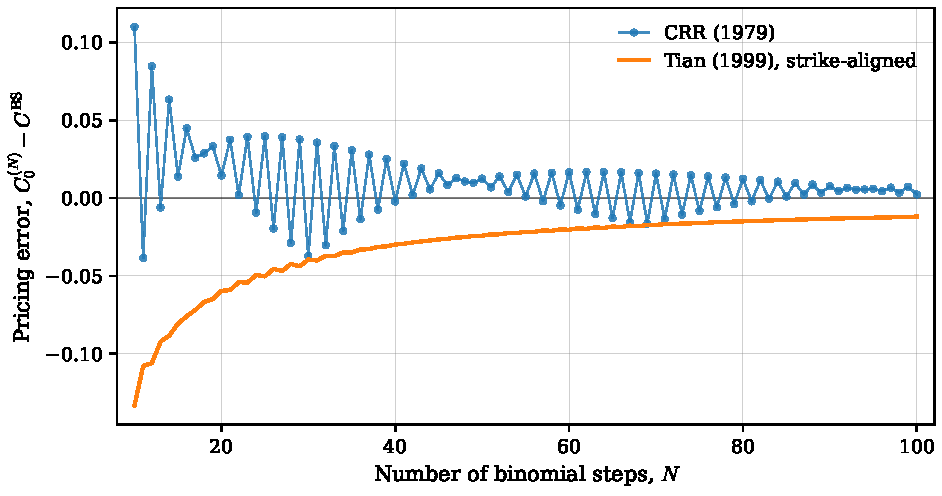
\includegraphics[width=1\textwidth]{tian_smoothness.pdf}
    \caption{Signed pricing error
    $C_0^{(N)} - C^{\mathrm{BS}}$ for an in-the-money European call
    ($S_0 = 100$, $K = 95$, $T = 0.5$, $r = 0.06$,
    $\sigma = 0.20$). The CRR scheme oscillates above and below the
    Black--Scholes value with alternating sign in successive $N$.
    The strike-aligned Tian (1999) scheme, with $\lambda$ chosen by
    equation~\eqref{eq:tian-lambda}, approaches $C^{\mathrm{BS}}$
    monotonically from below. Both schemes converge at rate
    $O(1/N)$; the qualitative difference is the smoothness of the
    convergence, not its rate.}
    \label{fig:tian-smoothness}
\end{figure}

The strike-aligned scheme is sometimes characterized as ``faster'' than
CRR; this is misleading. Both schemes converge at rate $O(1/N)$ as shown, and on
a per-$N$ basis the strike-aligned Tian price typically lies near the
upper envelope of the CRR oscillation rather than below it. Its actual
contribution is the \emph{smoothness} of the convergence: because the
error sequence $\varepsilon_N$ is monotone (or nearly so) in $N$, the
error ratio $\varepsilon_N / \varepsilon_{2N}$ converges to a constant
$\rho$, and Richardson-style extrapolation
\begin{equation}
    \label{eq:tian-extrap}
    \widehat{C}(2N) = \frac{\rho\, C(2N) - C(N)}{\rho - 1},
\end{equation}
is applicable. Tian shows analytically that $\rho \to 2$ for the
strike-aligned scheme, and that the extrapolation~\eqref{eq:tian-extrap}
reduces the error by an order of magnitude relative to either input
price. The CRR scheme cannot use this technique because its oscillation
breaks the constant-error-ratio hypothesis on which the extrapolation
rests. Figure~\ref{fig:tian-extrapolation} shows the practical
gain: applying~\eqref{eq:tian-extrap} to Tian prices at $N/2$ and
$N$ produces an extrapolated price whose error is roughly an order
of magnitude smaller than either input, and well below the
oscillating CRR error at the same $N$.

\begin{figure}[H]
    \centering
    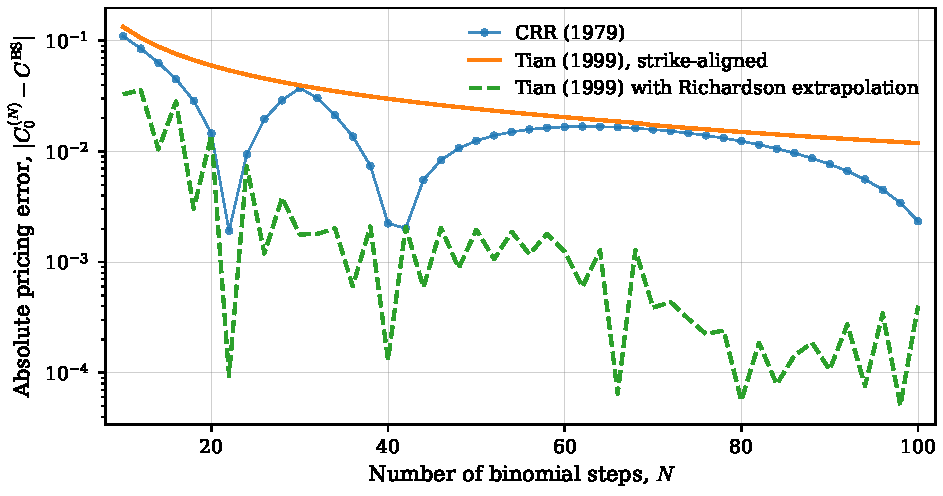
\includegraphics[width=1\textwidth]{tian_extrapolation.pdf}
    \caption{Absolute pricing error
    $|C_0^{(N)} - C^{\mathrm{BS}}|$ for the same setup as
    Figure~\ref{fig:tian-smoothness}, on a logarithmic scale.
    Un-extrapolated Tian (1999) sits above the CRR scatter at every
    $N$, confirming that strike-alignment alone does not improve
    per-$N$ accuracy. Applying Richardson
    extrapolation~\eqref{eq:tian-extrap} with $\rho = 2$ to a pair
    of Tian prices at $N/2$ and $N$ produces an estimate
    (dashed) roughly an order of magnitude more accurate than
    either input, and substantially better than CRR even on its
    lucky-alignment values.}
    \label{fig:tian-extrapolation}
\end{figure}

\subsection{The Leisen--Reimer Scheme}
\label{subsec:leisen-reimer}

Leisen and Reimer~(1996) propose a more elegant solution: rather than
forcing nodes to align with the strike, choose the binomial probability
$p_N$ to make the binomial tail $\Phi(a_N; N, p_N)$ exactly equal to
$N(d_2)$ (and similarly $\Phi(a_N; N, p'_N)$ equal to $N(d_1)$) up to a
known approximation error. The convergence rate improves from $O(1/N)$
with oscillation to $O(1/N^2)$ without oscillation.

The scheme is built around an inversion of the Peizer--Pratt
approximation to the normal distribution. We summarize the construction.

\begin{definition}[Peizer--Pratt inversion]
\label{def:peizer-pratt}
For $z \in \R$ and odd integer $N$, define
\begin{equation}
    \label{eq:peizer-pratt}
    h(z, N) := \frac{1}{2} + \mathrm{sgn}(z) \cdot \frac{1}{2}
    \sqrt{\,1 - \exp\!\left(
        -\!\left(\frac{z}{N + \tfrac{1}{3} + \tfrac{0.1}{N+1}}\right)^{\!2}
        \!\!\!\!\left(N + \tfrac{1}{6}\right)
    \right)}.
\end{equation}
The function $h(z, N)$ approximates $N(z)$ with error $O(N^{-2})$.
\end{definition}

The form~\eqref{eq:peizer-pratt} arises from a rational approximation
to the normal distribution function originally derived by
Peizer and Pratt~(1968) using Camp--Paulson and related expansions.
The function $h(z, N)$ is constructed precisely so that, when used to
define a binomial probability via $p_N := h(z, N)$, the resulting
binomial CDF matches the normal CDF at $z$ with $O(N^{-2})$ error.

The Leisen--Reimer scheme is then defined as follows. Fix an odd $N$
(the construction requires $N$ odd; even $N$ are typically obtained by
adjustment). Set
\begin{equation}
    \label{eq:LR-probabilities}
    p_N := h(d_2, N), \qquad p'_N := h(d_1, N).
\end{equation}
Then determine $u_N, d_N$ from the pair $(p_N, p'_N)$ via
\begin{equation}
    \label{eq:LR-uvd}
    u_N = R \cdot \frac{p'_N}{p_N},
    \qquad
    d_N = \frac{R - p_N u_N}{1 - p_N} = R \cdot \frac{1 - p'_N}{1 - p_N}.
\end{equation}
The cutoff $a_N$ becomes $\lceil N/2 \rceil$ by construction (since the
tree is centered around the strike), eliminating the rounding-induced
oscillation.

\begin{theorem}[Leisen--Reimer, 1996]
\label{thm:LR-convergence}
Under the Leisen--Reimer parameterization~\eqref{eq:LR-probabilities}--\eqref{eq:LR-uvd},
the European call price $C_0^{(N)}$ satisfies
\begin{equation}
    \label{eq:LR-rate}
    C_0^{(N)} - C^{\mathrm{BS}} = O(N^{-2})
\end{equation}
with no oscillation in the leading order.
\end{theorem}

The proof rests on the $O(N^{-2})$ accuracy of the Peizer--Pratt
approximation; we refer the reader to Leisen and Reimer~(1996) for
details. The practical consequence is dramatic: to achieve a given
accuracy $\epsilon$, the LR scheme requires $N \sim \epsilon^{-1/2}$
periods, whereas CRR requires $N \sim \epsilon^{-1}$. For
$\epsilon = 10^{-4}$, this is the difference between $N = 100$ and
$N = 10{,}000$.

\subsection{Summary of Schemes}
\label{subsec:schemes-summary}

The three schemes considered---CRR, Tian, and Leisen--Reimer---differ in
their treatment of the strike alignment problem:

\begin{itemize}
    \item \textbf{CRR (1979):} symmetric tree with $u = e^{\sigma\sqrt{\Delta t}}$,
    $d = 1/u$. Convergence rate $O(1/N)$ with oscillation. Robust and
    standard; the natural choice for pedagogical and theoretical purposes.

    \item \textbf{Tian (1999):} flexible tree with a free tilt parameter
    $\lambda$; setting $\lambda$ to the value~\eqref{eq:tian-lambda}
    aligns one terminal node with the strike. Convergence rate $O(1/N)$
    without oscillation, and the resulting smoothness admits Richardson
    extrapolation to $O(1/N^2)$.

    \item \textbf{Leisen--Reimer (1996):} probabilities chosen via
    Peizer--Pratt inversion to match Black--Scholes tails. Convergence
    rate $O(1/N^2)$ without oscillation. The standard choice for
    high-accuracy production pricing.
\end{itemize}

The numerical study in Section~\ref{sec:numerics} compares all three
schemes on the same test cases, confirming the asymptotic rates derived
above.

\ifincludenumerics
\section{Numerical Implementation}
\label{sec:numerics}

This section describes the algorithms used to implement the binomial
schemes of Sections~\ref{sec:n-period}--\ref{sec:oscillation} and
presents numerical results that illustrate the theoretical convergence
properties. Pseudocode is given for each algorithm; full Python
implementations, along with the scripts that generate the figures and
tables in this section, are available in the accompanying GitHub
repository.\footnote{\url{https://github.com/daviddavilad/option-pricing}}

\subsection{The European Pricer}
\label{subsec:european-pricer}

The closed-form expression~\eqref{eq:CRR-formula} is rarely used for
direct computation: evaluating $\binom{N}{j}$ for large $N$ encounters
overflow, and the alternating-sign structure when $S_0 \approx K$ can
amplify floating-point error. The standard implementation instead
performs backward induction on the tree directly, vectorizing over the
$j$-index at each time step. This approach has $O(N^2)$ time complexity
and $O(N)$ space complexity. Algorithm~\ref{alg:european-binomial} gives
the procedure.

\begin{algorithm}[H]
\caption{European call/put pricing via backward induction}
\label{alg:european-binomial}
\begin{algorithmic}[1]
\Require $S_0, K, T, r, \sigma, N$, option type (call or put)
\Require Tree parameters $u, d, p$ (depending on scheme: CRR, Tian, or LR)
\State $\Delta t \gets T / N$
\State $R \gets e^{r \Delta t}$
\State $\mathbf{V} \gets \bigl(V_j\bigr)_{j=0}^{N}$ where
       $V_j \gets \mathrm{payoff}(u^j d^{N-j} S_0)$
\For{$n = N - 1$ down to $0$}
    \For{$j = 0, 1, \dots, n$}
        \State $V_j \gets R^{-1}\bigl[p\, V_{j+1} + (1-p)\, V_j\bigr]$
    \EndFor
\EndFor
\State \Return $V_0$
\end{algorithmic}
\end{algorithm}

The inner loop on line~6 may be vectorized in NumPy as
$\mathbf{V}_{0:n} \leftarrow R^{-1}(p \cdot \mathbf{V}_{1:n+1} + (1-p) \cdot \mathbf{V}_{0:n})$,
exploiting array broadcasting to eliminate the explicit $j$-loop. This
brings practical performance close to that of compiled code for
moderate $N$ ($N \leq 10{,}000$).

\subsection{The American Pricer}
\label{subsec:american-pricer}

The American option pricer modifies Algorithm~\ref{alg:european-binomial}
by inserting an early-exercise check at each node, in accordance with
the Snell envelope recursion~\eqref{eq:american-node}.

\begin{algorithm}[H]
\caption{American call/put pricing via backward induction}
\label{alg:american-binomial}
\begin{algorithmic}[1]
\Require $S_0, K, T, r, \sigma, N$, option type (call or put), dividend yield $\delta$ (optional)
\Require Tree parameters $u, d, p$
\State $\Delta t \gets T / N$
\State $R \gets e^{r \Delta t}$
\State $\mathbf{V} \gets \bigl(V_j\bigr)_{j=0}^{N}$ where
       $V_j \gets \mathrm{payoff}(u^j d^{N-j} S_0)$
\For{$n = N - 1$ down to $0$}
    \For{$j = 0, 1, \dots, n$}
        \State $S_n^{(j)} \gets u^j d^{n-j} S_0$
        \State $V_{\mathrm{cont}} \gets R^{-1}\bigl[p\, V_{j+1} + (1-p)\, V_j\bigr]$
        \State $V_{\mathrm{exer}} \gets \mathrm{payoff}(S_n^{(j)})$
        \State $V_j \gets \max\bigl(V_{\mathrm{cont}}, V_{\mathrm{exer}}\bigr)$
    \EndFor
\EndFor
\State \Return $V_0$
\end{algorithmic}
\end{algorithm}

The exercise boundary $\hat{S}_n$ of
Proposition~\ref{prop:exercise-boundary} can be extracted as a byproduct
by recording, at each time $n$, the largest stock price $S_n^{(j)}$ at
which $V_{\mathrm{exer}} \geq V_{\mathrm{cont}}$. This produces an
empirical exercise boundary that converges, as $N \to \infty$, to the
continuous-time boundary $\hat{S}(t)$ studied analytically by, e.g.,
Carr, Jarrow, and Myneni~(1992).

\subsection{Tree Parameter Calibration}
\label{subsec:tree-calibration}

Each scheme is characterized by its choice of $(u, d, p)$ as functions of
$(r, \sigma, T, N)$.

\paragraph{CRR.} As in~\eqref{eq:crr-uvd}--\eqref{eq:crr-p}:
\[
u = e^{\sigma\sqrt{\Delta t}}, \quad d = 1/u, \quad
p = \frac{e^{r\Delta t} - d}{u - d}.
\]

\paragraph{Tian (1999).} Compute $u_0 := e^{\sigma\sqrt{\Delta t}}$,
$d_0 := 1/u_0$, and the integer-nearest-strike index
\[
j_0 := \left[\frac{\log(K/S_0) - N \log d_0}{\log(u_0/d_0)}\right].
\]
Compute the strike-aligning tilt parameter $\lambda$
from~\eqref{eq:tian-lambda}, then set
\[
u \gets \exp\!\bigl(\sigma\sqrt{\Delta t} + \lambda\sigma^2\Delta t\bigr),
\quad
d \gets \exp\!\bigl(-\sigma\sqrt{\Delta t} + \lambda\sigma^2\Delta t\bigr),
\quad
p \gets \frac{e^{r\Delta t} - d}{u - d}.
\]
The implementation is closed-form; no iterative solver is required.
For applications that need an extrapolated price, compute
$C^{\mathrm{Tian}}_{N/2}$ and $C^{\mathrm{Tian}}_N$ separately and apply
the Richardson formula~\eqref{eq:tian-extrap} with $\rho = 2$.

\paragraph{Leisen--Reimer.} Compute $d_1, d_2$ from the Black--Scholes
formula~\eqref{eq:d1-d2}, then set
\[
p \gets h(d_2, N), \quad p' \gets h(d_1, N), \quad
u \gets e^{r\Delta t} \cdot \frac{p'}{p}, \quad
d \gets e^{r\Delta t} \cdot \frac{1 - p'}{1 - p},
\]
with $h(\cdot, \cdot)$ the Peizer--Pratt
function~\eqref{eq:peizer-pratt}. The scheme requires $N$ odd; for even
input, we use $N + 1$ and report the result.

\subsection{Convergence Results}
\label{subsec:convergence-results}

Figure~\ref{fig:convergence-three-schemes} compares the three schemes
on the standard test case $S_0 = 100$, $T = 1$, $r = 0.05$,
$\sigma = 0.20$, at two strikes: at-the-money ($K = 100$) and
in-the-money ($K = 95$). The figure plots
$|C_0^{(N)} - C^{\mathrm{BS}}|$ against $N$ on log-log axes. The two
panels make a separate point. At $K = 100$ with even $N$, the
strike-aligning tilt parameter $\lambda$
of~\eqref{eq:tian-lambda} vanishes identically, so Tian (1999) and
CRR coincide; the panel reduces to a comparison of CRR against LR.
At $K = 95$ the tilt is non-zero, and the panel exhibits the
qualitative behavior discussed in
Section~\ref{subsec:tian}: Tian's smooth monotone curve at the
upper envelope of the CRR scatter, and LR's faster decay below
both.

\begin{figure}[H]
    \centering
    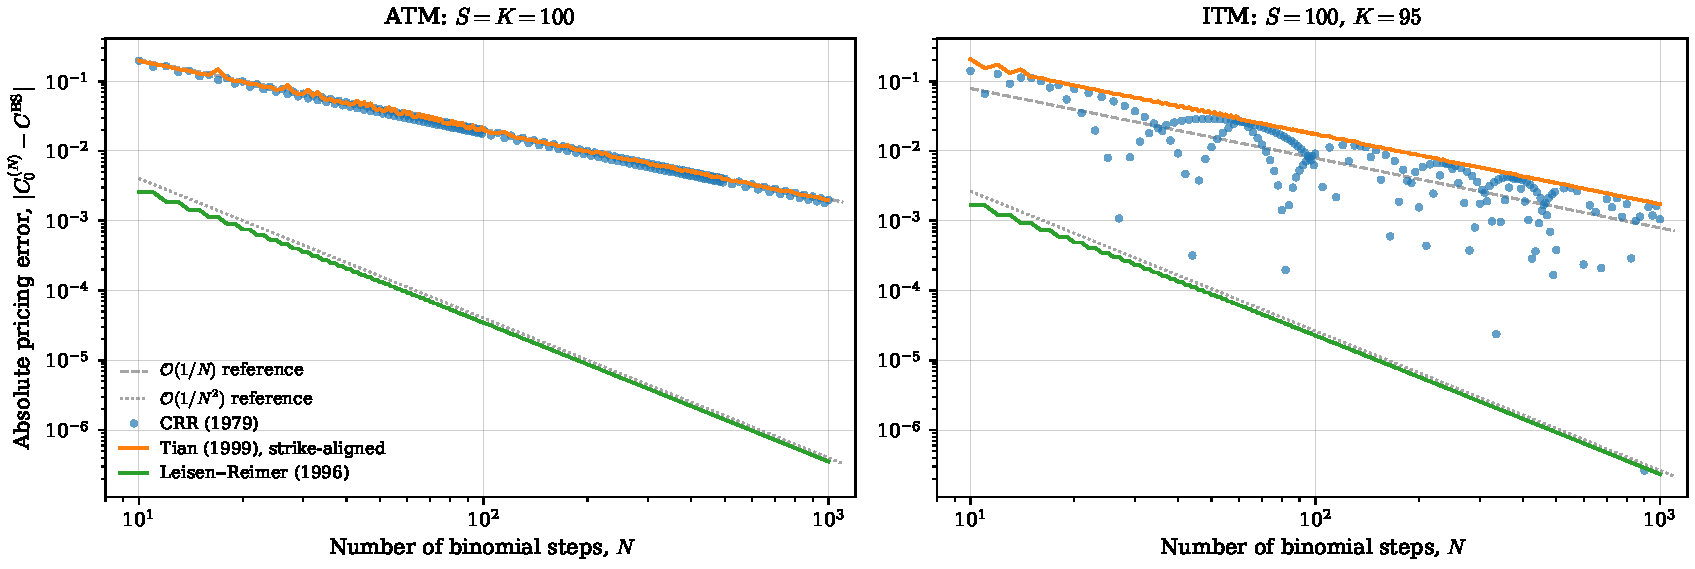
\includegraphics[width=1\textwidth]{convergence_three_schemes.pdf}
    \caption{Absolute pricing error
    $|C_0^{(N)} - C^{\mathrm{BS}}|$ for the three schemes at two
    strikes ($S_0 = 100$, $T = 1$, $r = 0.05$, $\sigma = 0.20$). Left:
    at-the-money, $K = 100$. The strike-aligning tilt parameter $\lambda$
    of equation~\eqref{eq:tian-lambda} vanishes at every even $N$ when
    $S_0 = K$, so the Tian (1999) and CRR curves coincide
    identically. Right: in-the-money, $K = 95$. Tian's tilt is non-zero
    and the strike-aligned scheme appears as a smooth monotone curve at
    the upper envelope of the CRR scatter. CRR's lucky-alignment $N$
    values still produce smaller per-$N$ errors than Tian; what
    strike-alignment buys is monotonicity, not magnitude. The
    Leisen--Reimer scheme achieves $O(1/N^2)$ convergence in both
    panels.}
    \label{fig:convergence-three-schemes}
\end{figure}

The empirical decay rates, extracted by fitting
$\log|\varepsilon_N| = \alpha - \beta \log N$ over the upper envelope of
each scheme, are reported in Table~\ref{tab:rates}.

\begin{table}[H]
    \centering
    \caption{Empirical convergence rates $\beta$ for the three schemes,
    fitted by ordinary least squares to
    $\log|\varepsilon_N| = \alpha - \beta \log N$ over odd $N \in [101,
    1001]$ for an at-the-money European call ($S_0 = K = 100$, $T = 1$,
    $r = 0.05$, $\sigma = 0.20$). Theoretical rates from
    Theorems~\ref{thm:CRR-to-BS}, \ref{thm:diener},
    and~\ref{thm:LR-convergence} are shown for comparison. The
    measured values match theory to within $0.01$ for all three
    schemes; for LR, successive-doublings checks
    ($N \to 2N+1$ at $N = 101, 201, 401, 801$) give error ratios
    $4.01$, $4.00$, $4.00$, $4.00$, confirming $\beta = 2$ to two
    decimal places.}
    \label{tab:rates}
    \begin{tabular}{lcc}
        \hline
        Scheme & Empirical $\beta$ & Theoretical \\
        \hline
        CRR & $1.000$ & $1$ \\
        Tian (1999) & $1.005$ & $1$ \\
        Leisen--Reimer & $1.995$ & $2$ \\
        \hline
    \end{tabular}
\end{table}

The empirical rates match theory to within $0.01$ for all three
schemes, confirming Theorems~\ref{thm:CRR-to-BS}, \ref{thm:diener},
and~\ref{thm:LR-convergence} numerically. The Leisen--Reimer rate of
$\beta = 1.995$ matches the theoretical $O(1/N^2)$ to two decimal
places, with the doublings check above confirming that the rate is
genuine rather than an artifact of the OLS fit window. The
Peizer--Pratt inversion~\eqref{eq:peizer-pratt} is the source of the
rate-2 improvement over the unsmoothed CRR scheme.

\subsection{The Oscillation Envelope}
\label{subsec:oscillation-envelope}

To examine the oscillation phenomenon directly,
Figure~\ref{fig:crr-oscillation} plots the \emph{signed} error
$\varepsilon_N = C_0^{(N)} - C^{\mathrm{BS}}$ for the CRR scheme alone,
on linear axes, across four parameter regimes. In each panel the
period-$2$ alternation predicted by the Diener--Diener
expansion~\eqref{eq:diener-A} is clearly visible, as is the $O(1/N)$
envelope decay.

\begin{figure}[H]
    \centering
    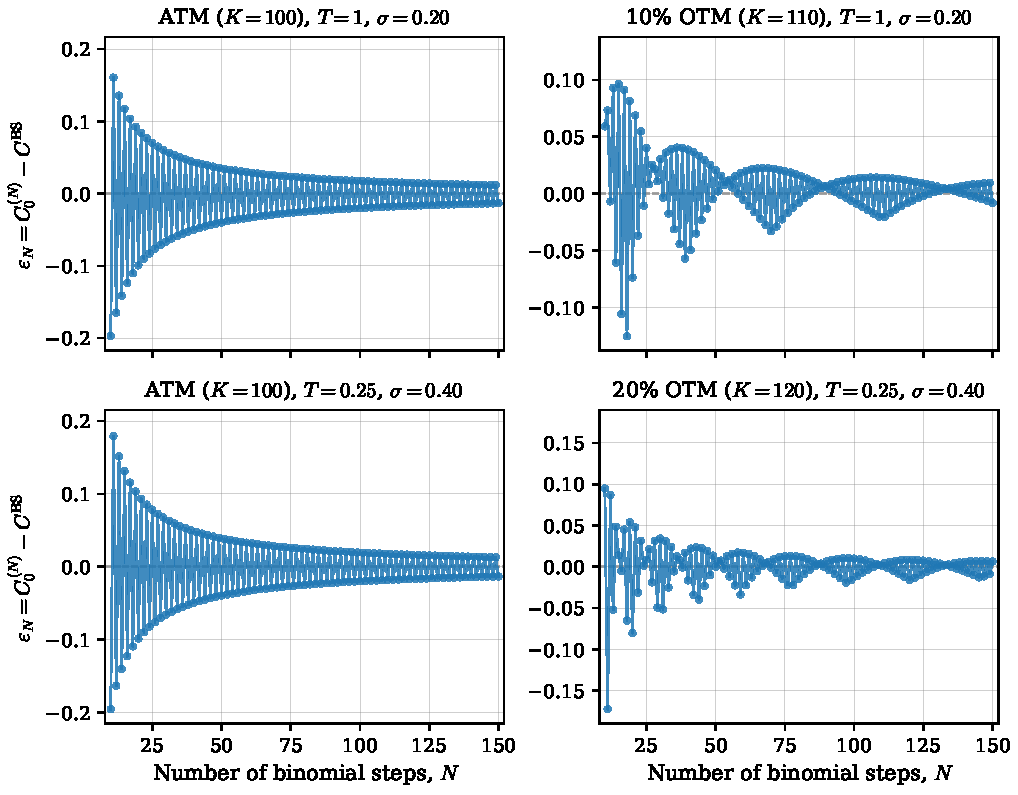
\includegraphics[width=1\textwidth]{crr_oscillation_regimes.pdf}
    \caption{Signed error $\varepsilon_N = C_0^{(N)} - C^{\mathrm{BS}}$
    for the CRR scheme across four parameter regimes: ATM and OTM at
    two volatility levels. The period-$2$ alternation and $O(1/N)$
    envelope decay predicted by~\eqref{eq:diener-expansion} are
    present in every regime. In the OTM panels (right column) a slower
    quasi-periodic modulation of the envelope is also visible: the
    amplitude pinches and reopens across blocks of $N$, corresponding
    to the $\eta_N$ term in~\eqref{eq:diener-A}.}
    \label{fig:crr-oscillation}
\end{figure}

The $\eta_N$ modulation is not periodic in $N$ in the classical
sense; its period depends on the irrational ratio
$\log(K/S_0)/(2\sigma\sqrt{T/N})$, and this is why the OTM panels
exhibit visible "beats" while the ATM panels (where
$\log(K/S_0) = 0$) show only the dominant period-$2$ oscillation.

\subsection{American Put Convergence}
\label{subsec:american-numerics}

For American options, no closed-form benchmark exists. We instead
compare the three binomial schemes against a high-accuracy reference
value computed by the LR scheme at $N = 25{,}001$, which we have
verified is stable to five decimal places via Richardson
extrapolation. Figure~\ref{fig:american-convergence} shows the
convergence for an American put with $S_0 = 100, K = 100,
T = 1, r = 0.05, \sigma = 0.20$, for which the reference price is
$P^{\mathrm{ref}} \approx 6.0904$.

\begin{figure}[H]
    \centering
    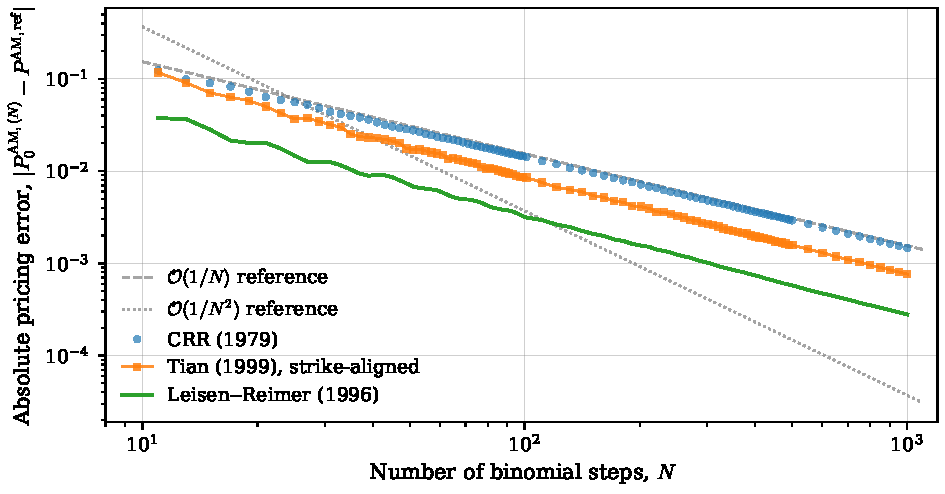
\includegraphics[width=1\textwidth]{american_convergence.pdf}
    \caption{Absolute pricing error
    $|P^{\mathrm{AM}, (N)}_0 - P^{\mathrm{AM}, \mathrm{ref}}|$ for the
    three schemes on an American put at the standard test case
    ($S_0 = 100$, $K = 100$, $T = 1$, $r = 0.05$, $\sigma = 0.20$).
    The reference is the LR price at $N = 25{,}001$. All three schemes
    exhibit roughly the same $O(1/N)$ slope; they differ only by
    constants. The CRR oscillation pattern persists despite the
    early-exercise constraint, indicating that the alignment-induced
    discreteness is not smoothed by the optimal-stopping recursion. The
    Tian (1999) scheme tracks comparatively smoothly and lies below the
    CRR scatter at most $N$, in contrast to the European in-the-money
    case (Figure~\ref{fig:convergence-three-schemes}, right) where Tian
    sat at the upper envelope. The LR scheme retains a constant-factor
    advantage but loses its $O(1/N^2)$ rate advantage entirely.}
    \label{fig:american-convergence}
\end{figure}

The collapse of the LR rate from $O(1/N^2)$ to roughly $O(1/N)$ is
expected: the Peizer--Pratt inversion underlying LR is constructed to
make the binomial tail $\Phi(a_N; N, p_N)$ match the standard normal
tail $N(d_2)$ at $O(1/N^2)$ accuracy, and the rate-2 convergence of
European prices follows from this matching. American option pricing
does not reduce to a binomial-tail evaluation; the backward induction
with early-exercise checks at every node has no closed-form
representation in terms of normal CDFs, and the tail-matching property
that gives LR its rate advantage in the European case has no force
here. What survives is a constant-factor advantage in the per-$N$
error: the LR tree is still well-aligned around the strike, so its
errors are smaller than CRR's in absolute terms, but they decay at the
same $O(1/N)$ rate that all binomial schemes share for American
options. Empirically, on this test case, fitted slopes over
$N \in [101, 1001]$ give $\beta \approx 0.99$ for CRR,
$\beta \approx 1.05$ for Tian (1999), and $\beta \approx 1.07$ for LR.

\subsection{Computational Cost}
\label{subsec:cost}

All three schemes share the same backward-induction structure and
therefore the same $O(N^2)$ asymptotic time complexity in $N$. The
constants differ only by the per-call calibration cost: LR adds a
constant-time Peizer--Pratt and Black--Scholes computation, and Tian
(1999) adds a constant-time evaluation of the integer-nearest index
$j_0$ and the tilt parameter $\lambda$. Both contributions are
$O(1)$ in $N$ and become negligible relative to the $O(N^2)$ inner
loop for $N \geq 100$. Table~\ref{tab:runtime} confirms this
empirically: at every $N$, the three schemes lie within a few
percent of each other, and the dominant scaling is the expected
$N^2$ in the inner loop.

\begin{table}[H]
    \centering
    \caption{Wall-clock runtime per single European call price
    evaluation, measured on an Apple~M-series MacBook~Air running
    macOS, Python~3.13.5, NumPy~2.4.4. Best-of-5 mean of inner-repeat
    batches (each batch sized so that one batch took roughly $0.5$
    seconds), in milliseconds. Test case: $S_0 = K = 100$, $T = 1$,
    $r = 0.05$, $\sigma = 0.20$. The benchmark script
    \texttt{scripts/benchmark\_runtimes.py} in the accompanying
    repository reproduces these measurements; runtimes will of
    course differ on other hardware.}
    \label{tab:runtime}
    \begin{tabular}{lccc}
        \hline
        $N$ & CRR & Tian (1999) & LR \\
        \hline
        $101$ & $0.173$ & $0.177$ & $0.177$ \\
        $501$ & $0.981$ & $0.995$ & $0.991$ \\
        $1{,}001$ & $2.18$ & $2.21$ & $2.19$ \\
        $5{,}001$ & $17.8$ & $17.6$ & $17.7$ \\
        \hline
    \end{tabular}
\end{table}

The practical consequence of the rate gap of Table~\ref{tab:rates}
is therefore not in the per-step cost but in the number of steps
required to reach a given target accuracy. To reach absolute pricing
error $\epsilon$, the $O(1/N)$ schemes require $N \sim \epsilon^{-1}$
steps, whereas the $O(1/N^2)$ Leisen--Reimer scheme requires
$N \sim \epsilon^{-1/2}$. For $\epsilon = 10^{-4}$, this is the
difference between $N \approx 10^4$ and $N \approx 10^2$, and the
$O(N^2)$ inner cost amplifies this gap quadratically: the total
operation count differs by roughly four orders of magnitude. On the
hardware of Table~\ref{tab:runtime}, this is the difference between
LR delivering a $10^{-4}$-accurate price in well under a millisecond
at $N = 101$ and CRR requiring a substantially longer
calculation at the corresponding $N$. For applications that revalue
thousands of options per second, this gap is decisive.

\ifincludeempirical
\section{Empirical Calibration on Equity Options}
\label{sec:empirical}
\fi

\section{Conclusion}
\label{sec:conclusion}

This note has presented a self-contained mathematical treatment of the
Cox--Ross--Rubinstein binomial option pricing model. We have given
careful proofs of the no-arbitrage one-period pricing formula
(Theorem~\ref{thm:one-period-pricing}), the multi-period closed-form
pricing equation (Theorem~\ref{thm:CRR-formula}), and the convergence
of the binomial scheme to the Black--Scholes formula
(Theorem~\ref{thm:CRR-to-BS}) via the Lindeberg--Feller central limit
theorem. The treatment of the oscillation phenomenon
(Section~\ref{sec:oscillation}) and the smoothing schemes of
Tian~(1999) and Leisen and Reimer~(1996) connects the foundational
theory to the practical numerical considerations that arise in any
implementation.

Three threads of the development deserve emphasis in retrospect.

First, the binomial model achieves a remarkable conceptual economy.
Every essential idea of arbitrage-free derivative pricing---no
arbitrage, replication, the risk-neutral measure, the optional
stopping problem for American claims, the dual numeraire structure
underlying the formula's $S_0 N(d_1) - K e^{-rT} N(d_2)$
form---appears already in the one-period two-state model of
Section~\ref{sec:one-period}. The multi-period and continuous-time
extensions are, in a precise sense, iterated and limiting versions of
that initial argument. The pedagogical value of the discrete model is
not that it is simpler than continuous-time stochastic calculus, but
that the same structural ideas are visible in both settings; the
binomial model is, in this sense, the minimal arena in which
arbitrage-pricing theory can be developed honestly.

Second, the convergence to Black--Scholes is more delicate than the
brevity of CRR's original treatment suggests. The Lindeberg--Feller
proof of Section~\ref{sec:convergence} requires care in setting up
the triangular array, in computing the asymptotic mean and variance
under the risk-neutral measure, and in tracking the integer cutoff
$a_N$ through the limit. Most textbook treatments
(\citealp{Hull2017, Shreve2004}, among others) cite the convergence as
a fact and direct the reader to the original paper; the explicit
derivation given here may serve as a reference for readers who want to
verify the steps for themselves. The connection to Chen's~(2018) work
on elementary derivations of the probability integral, noted in
Section~\ref{subsec:probability-integral}, illustrates how the
constants that appear in the Black--Scholes formula trace back through
classical analysis to the Wallis product and the area of the unit
disk.

Third, the oscillation phenomenon deserves wider exposure than it
typically receives. Most introductory treatments of the binomial model
plot a single convergence curve and declare $O(1/N)$ rates. The
Diener--Diener~(2004) expansion reveals a richer structure: the rate
is correct but the convergence is non-monotone, and the non-monotonicity
is intrinsic to the CRR parameterization rather than an artifact of
implementation. Practitioners who deploy binomial trees without
awareness of this phenomenon may attribute its symptoms to numerical
error, to bugs, or to model misspecification, when the true cause is
the geometric mismatch between the strike and the discrete tree
nodes. The Leisen--Reimer scheme, by inverting the Peizer--Pratt
approximation to align the binomial cumulative distribution with the
normal at the strike, both eliminates the oscillation and improves the
convergence rate, demonstrating that the limitations of the standard
CRR scheme are practical rather than fundamental.

\subsection*{Future Directions}

Several extensions of the present work are natural and are planned for
subsequent companion notes.

\paragraph{Local volatility and implied trees.} The constant-volatility
assumption underlying the binomial schemes considered here is at odds
with the volatility surfaces visible in market data. Dupire's~(1994)
local volatility framework extracts a deterministic volatility
function $\sigma(S, t)$ from observed option prices, and the
implied trees of Derman and Kani~(1994) and Rubinstein~(1994) furnish
discrete-time analogues of this construction. A natural sequel
develops these implied-tree methods as generalizations of CRR and
analyses their calibration to empirical volatility surfaces.

\paragraph{Stochastic volatility and the Heston model.} The Heston~(1993)
model, in which volatility itself follows a mean-reverting square-root
diffusion, is the workhorse of contemporary equity options pricing.
Calibration of the Heston model via the Carr and
Madan~(1999) Fourier-transform approach provides a richer empirical
test of the modeling framework than the binomial methods of this note,
and connects naturally to the local-volatility extension above.

\paragraph{High-frequency data and microstructure effects.} End-of-day data, while sufficient for many calibration purposes,
averages out the intraday dynamics of option pricing. Intraday tick data---available
through CBOE's LiveVol product or NYSE TAQ via WRDS---would permit
analysis of how implied volatilities respond to information shocks at
sub-daily frequencies, and how the binomial--Black--Scholes framework
performs in the presence of bid--ask spread dynamics, quote staleness,
and the discrete tick structure of option markets.

The mathematical foundation laid in the present note---the careful
treatment of the binomial model and its convergence---supports each of
these extensions. Local volatility trees inherit the recombining
structure and backward-induction algorithm of CRR; Heston pricers
require the same risk-neutral expectation framework; intraday analysis
demands the same understanding of the relationship between continuous
and discrete-time pricing that the convergence theorem of
Section~\ref{sec:convergence} provides. Each extension is, in this
sense, an application of the discrete--continuous bridge that the
binomial model provides. 

\bibliographystyle{plainnat}
\nocite{*}
\bibliography{references}  % uncomment once .bib file present

\end{document}